\documentclass[a4paper,11pt]{article}
\usepackage[ansinew]{inputenc} 
\usepackage[T1]{fontenc}
\usepackage{tikz}
\usetikzlibrary{calc,patterns,angles,quotes}
\usepackage{ae,amsmath,amssymb,amsthm}
\usepackage[english]{babel}
%\usepackage[portuguese]{babel}
\usepackage{graphicx}
\usepackage{color}
\usepackage{subcaption}
\usepackage{setspace} 
\usepackage{float}
\usepackage[sc]{titlesec}
%\oddsidemargin 0.22in
\textwidth 5.8in
\parindent 10mm
\usepackage{url,hyperref}

\hypersetup{
     colorlinks = true,
     linkcolor = black,
     citecolor=blue,
}
\usepackage{comment}  
\usepackage{listings}

\lstset{
    backgroundcolor=\color[rgb]{0.86,0.88,0.93},
    language=Python, %keywordstyle=\color[rgb]{0.1,0,1},
    basicstyle=\footnotesize \ttfamily,breaklines=true, numbers=left,
    escapeinside={\%*}{*)}
}

\oddsidemargin 10pt
\textwidth 445pt
\textheight 650pt
\topmargin = -25pt

%%%%%%%%%% Cover page %%%%%%%%%%%
\begin{document}
\begin{figure}[!h] 
\includegraphics [scale=0.35] {Figures/FromMichela/Course-logo-long} \end{figure}

\begin{spacing}{1.5}
{\Large\sc \noindent TI0118 -- Homework 1} \\

{\large\sc \noindent Student name: Emmanuel Victor Barbosa Sampaio}\\
{\large\sc \noindent Student number: 417180 }
\end{spacing}
\vskip1cm
%%%%%%%%%% Content starts %%%%%%%%%%%
\section*{Exercise 1}
Consider the two tanks system arranged as shown in Figure \ref{fig:ex1}.
\begin{figure}[H]
\begin{center}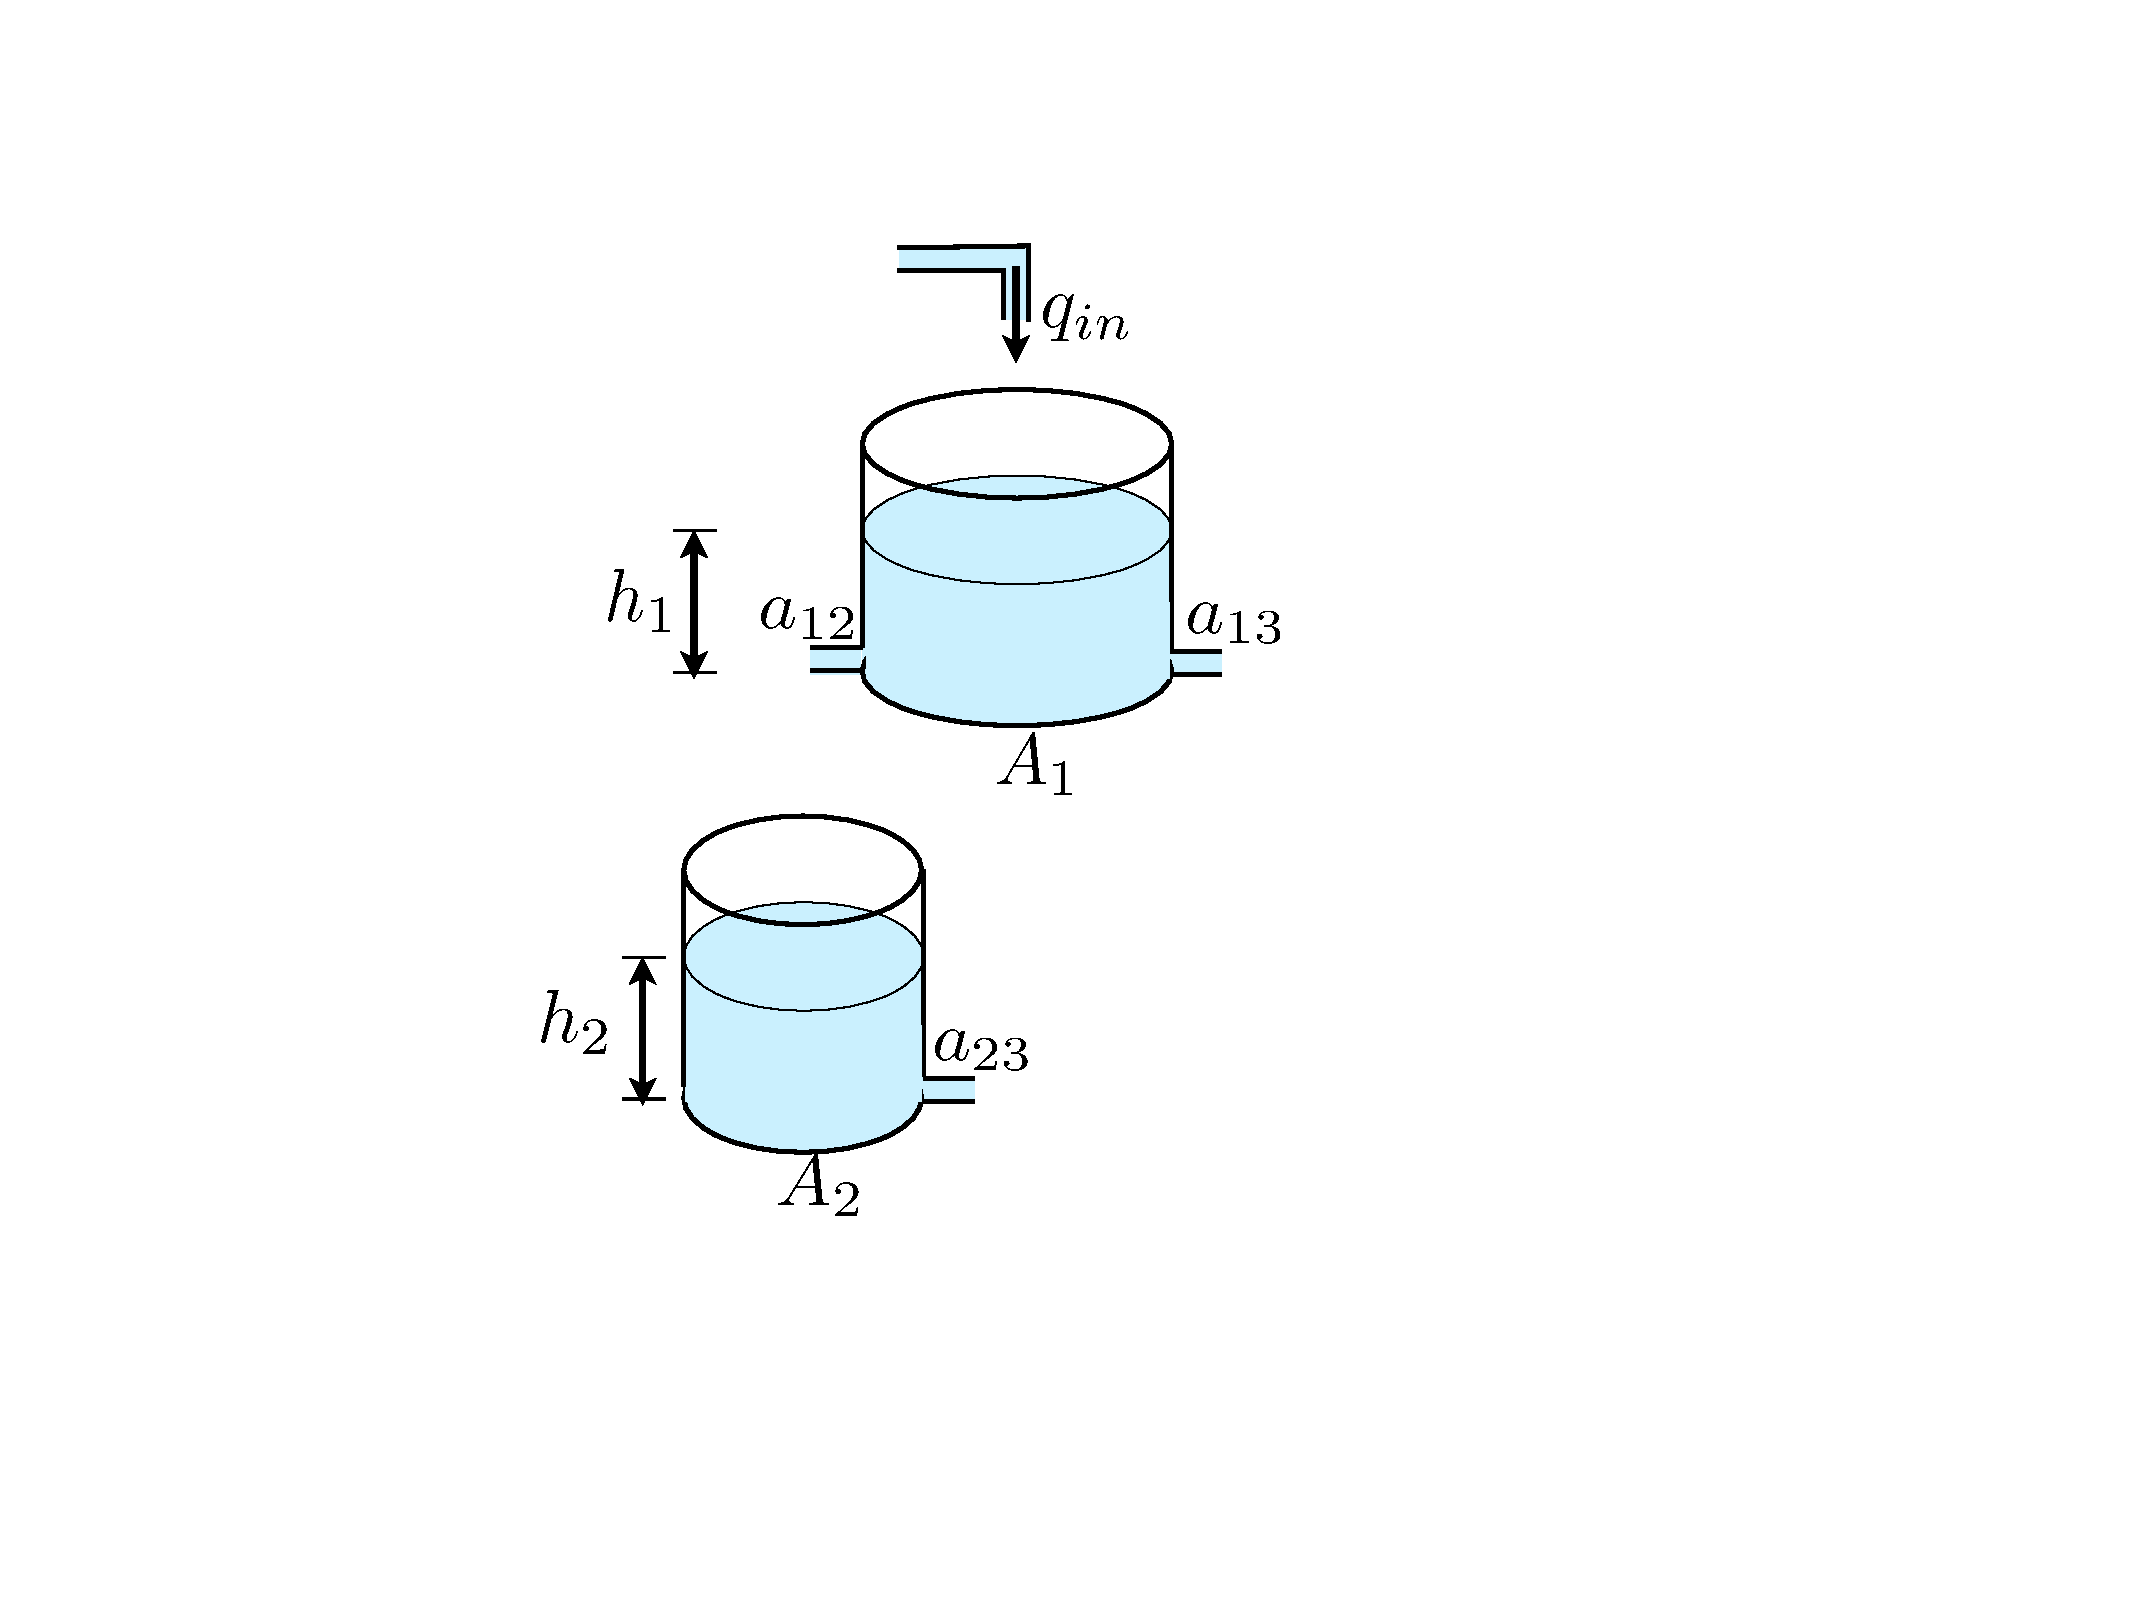
\includegraphics[width=0.31\textwidth]{Figures/FromMichela/tanks_ex} \end{center}
 \vskip-0.5cm\caption{Two-tank system for Exercise 1.}
\label{fig:ex1}
\end{figure}
\noindent The manipulated variable (input) is the volume flow rate $q_{in}$, while the measured variable (output) is the fluid level $h_2$ in the second tank.
 The areas of the two tanks are  $A_1$ and $A_2$, while $a_{12}, a_{13}$ and $a_{23}$ are the areas of the orifices indicated in Figures \ref{fig:ex1}. The fluid is perfect (no shear stresses, no viscosity, no heat conduction), and subject only to gravity\footnote{Hint: The flow rate is given by the Torricelli law: $q_i(t)=a_{i,j}\sqrt{2gh_i(t)}$}. The tanks are filled with water (incompressible fluid), and the external pressure is constant (atmospheric pressure).

\begin{enumerate}
\item Obtain a state-space model of the systzem, where $x_1(t)=h_1(t)$ and $x_2(t)=h_2(t)$ are state variables, $u(t)=q_{in}(t)$ is the input and $y(t)=h_2(t)$ is the output. 
\item Given $a_{12}=a_{23}=a_{13}= 1$ m$^2$, $A_1=200$ m$^2$, $A_2=200$ m$^2$, find the equilibrium state $(\bar{x}_1,\bar{x}_2)$ obtained with a constant input $\bar{u}=10$ m$^3/$s, approximating gravity acceleration as $g\approx 10$ m/s$^2$.
\item Determine the linearized system $(\mathbf{A},\mathbf{B},\mathbf{C},\mathbf{D})$ around the equilibrium state $(\bar{x}_1,\bar{x}_2)$.
\item In the programming language of your choice, simulate\footnote{Hint: In Matlab/Octave you can use the command {\tt lsim} to simulate the linear system and {\tt ode45} to simulate the non-linear system. Similarly, in Python you might use, respectively, {\tt control.matlab.lsim} and {\tt integrate.ode} specifying the integration method.} the two systems response to a unit input step \footnote{Hint: In Matlab/Octave you might use the {\tt step} command and {\tt control.matlab.step} in Python.} and discuss your results.
\end{enumerate}
\subsection*{Solution} 					
\par For the first tank, the equation that describes the variation of the level in the time is:
\begin{align}
\label{eq:Eq1}
A_1\frac{dh_1(t)}{dt}= q_{in}- q_{12}-q_{13}
\end{align}
\par For the second tank, the equation that describes the variation of the level in the time is:
\begin{align}
\label{eq:Eq2}
A_2\frac{dh_2(t)}{dt}= q_{12}-q_{23}
\end{align}
\par We can represent $q_{12}$, $q_{13}$, $q_{23}$ using Torricelli's law:
\begin{align*}
q_{12} &= a_{12}\sqrt{2gh_1(t)}\\
q_{13} &= a_{13}\sqrt{2gh_1(t)}\\
q_{23} &= a_{23}\sqrt{2gh_2(t)}\\
\end{align*}
\par Replacing in \ref{eq:Eq1} and \ref{eq:Eq2}:
\begin{align}
\label{eq:Eq3}
\frac{dh_1(t)}{dt} &= \frac{1}{A_1}q_{in}-\frac{1}{A_1}a_{12}\sqrt{2gh_1}-\frac{1}{A_1}a_{13}\sqrt{2gh_1}\\
\label{eq:Eq4}
\frac{dh_2(t)}{dt} &= \frac{1}{A_2}a_{12}\sqrt{2gh_1}-\frac{1}{A_2}a_{23}\sqrt{2gh_2}
\end{align}
\par The above equations describe the system behavior, but they are non-linear, as we want to represent the system using the state space model, we need to linearize these equations. To perform linearization, we can use Taylor's series to approximate the above functions to a linear model, using as a domain of the function the neighborhood of a point called a stationary point, at that point, the function is equal to zero. So, considering $ x_s $ as the stationary point Taylor's series for the function going to be represent as follows:
\begin{align*}
f(x) = f(x_s)+ (x-x_s)\frac{df(x)}{dx}\Big\vert_{x=x_s}+ \sum_{n=2}^\infty\frac{1}{n!}\frac{d^nf(x)}{dx^n}\Big\vert_{x=x_s}(x-x_s)^n
\end{align*}
\par $f(x_s)=0$, because $x_s$ is the stationary point. From the neighborhood condition, we can approximate $ (x-x_s) ^ n \; \forall n \geq 2 $ to zero. In conclusion the function approximation is:
\begin{align}
\label{eq:Eq5}
f(x) = (x-x_s)\frac{df(x)}{dx}\Big\vert_{x=x_s}
\end{align}
\par Based on what was explained, the first step of the linearization process is to find a stationary point. The equations \eqref{eq:Eq3} and \eqref{eq:Eq4} have as variables: the input $q_{in}$,the level of the first tank $h_1$ and the level of the second tank $h_2$, so we need to find the values of these variables in the stationary condition, which means, find the values where functions are represented as follows:
\begin{align*}
0 &=  q_{in}-a_{12}\sqrt{2gh_1}-a_{13}\sqrt{2gh_1}\\
0 &= a_{12}\sqrt{2gh_1}-a_{23}\sqrt{2gh_2}
\end{align*}
\par We can use the information that $a_{12}=a_{13}=a_{23}$:
\begin{align*}
q_{in} &= 2(a_{13}\sqrt{2gh_1})\\
\sqrt{2gh_1}&=\sqrt{2gh_2}\\
\end{align*}
\par Then:
\begin{align*}
\frac{q_{in}^2}{8ga_{13}^2}&=h_1\\
\frac{q_{in}^2}{8ga_{13}^2}&=h_2
\end{align*}
\par Using the information provided by the question about the input, we found the following values for $h_1,h_2$:
\begin{align}
\frac{10}{8}=1.25=h_1=h_2
\end{align}
\par In conclusion the stationary point is: $x_s=(1.25,1.25,10)$
\par Representing \eqref{eq:Eq3} and \eqref{eq:Eq4} as functions:
\begin{align}
\label{eq:Eq6}
\frac{dh_1(t)}{dt}&=f_1(h_1(t),h_2(t),q_{in}(t))= \frac{1}{A_1}(q_{in}-a_{12}\sqrt{2gh_1(t)}-a_{13}\sqrt{2gh_1(t)})\\
\label{eq:Eq7}
\frac{dh_2(t)}{dt}&=f_2(h_1(t),h_2(t),q_{in}(t))= \frac{1}{A_2}(a_{12}\sqrt{2gh_1(t)}-a_{23}\sqrt{2gh_2(t)})
\end{align}
\par Taking the partial derivative of \eqref{eq:Eq6}:
\begin{align*}
\frac{\partial f_1(h_1(t),h_2(t),q_{in}(t))}{\partial h_1}&= \frac{1}{A_1}\frac{\partial(-2a_{12}\sqrt{2gh_1(t)})}{\partial h_1}=\frac{-2a_{12}g}{
A_1\sqrt{2gh_1}}=0.02\\
\frac{\partial f_1(h_1(t),h_2(t),q_{in}(t))}{\partial h_2}&=0\\
\frac{\partial f_1(h_1(t),h_2(t),q_{in}(t))}{\partial q_{in}}&=\frac{1}{A_1}=0.005
\end{align*}
\par Taking the partial derivative of \eqref{eq:Eq7}:
\begin{align*}
\frac{\partial f_2(h_1(t),h_2(t),q_{in}(t))}{\partial h_1}&= \frac{1}{A_2}\frac{\partial(a_{12}\sqrt{2gh_1(t)})}{\partial h_1}=\frac{a_{12}g}{
A_2\sqrt{2gh_1}}=0.01\\
\frac{\partial f_2(h_1(t),h_2(t),q_{in}(t))}{\partial h_2}&= \frac{1}{A_2}\frac{\partial(-a_{23}\sqrt{2gh_2(t)})}{\partial h_2}=\frac{-a_{23}g}{
A_2\sqrt{2gh_2}}=-0.01\\
\frac{\partial f_2(h_1(t),h_2(t),q_{in}(t))}{\partial q_{in}}&=0
\end{align*}
\par Now using the Taylor's series expansion:
\begin{align*}
\frac{dh_1(t)}{dt}&=-0.02(h_1(t)-1.25)+0(h_2(t)-1.25)+0.005(q_{in}-10)\\
\frac{dh_2(t)}{dt}&=0.01(h_1(t)-1.25)-0.01(h_2(t)-1.25)
\end{align*}
\par The last equations are linear, then we can use the state space model representation:
\begin{align}
\label{eq:Eq8}
\begin{bmatrix}
\frac{d h_1}{dt}\\
\frac{d h_2}{dt}
\end{bmatrix}&=\begin{bmatrix}
-0.02 & 0\\
0.01 & -0.01\\
\end{bmatrix}\begin{bmatrix}
h_1(t) - 1.25\\
h_2(t) -1.25
\end{bmatrix}
+\begin{bmatrix}
0.005\\
0
\end{bmatrix}(q_{in}(t)-10)\\
y(t) &= \begin{bmatrix}
0& 1
\end{bmatrix}\begin{bmatrix}
h_1(t)-1.25\\
h_2(t)-1.25
\end{bmatrix}
\end{align}
\par Using the developed model and the nonlinear equation of $h_2(t)$ we can simulate the system output behavior due to a step with magnitude 10.
\begin{figure}[H]
\centering
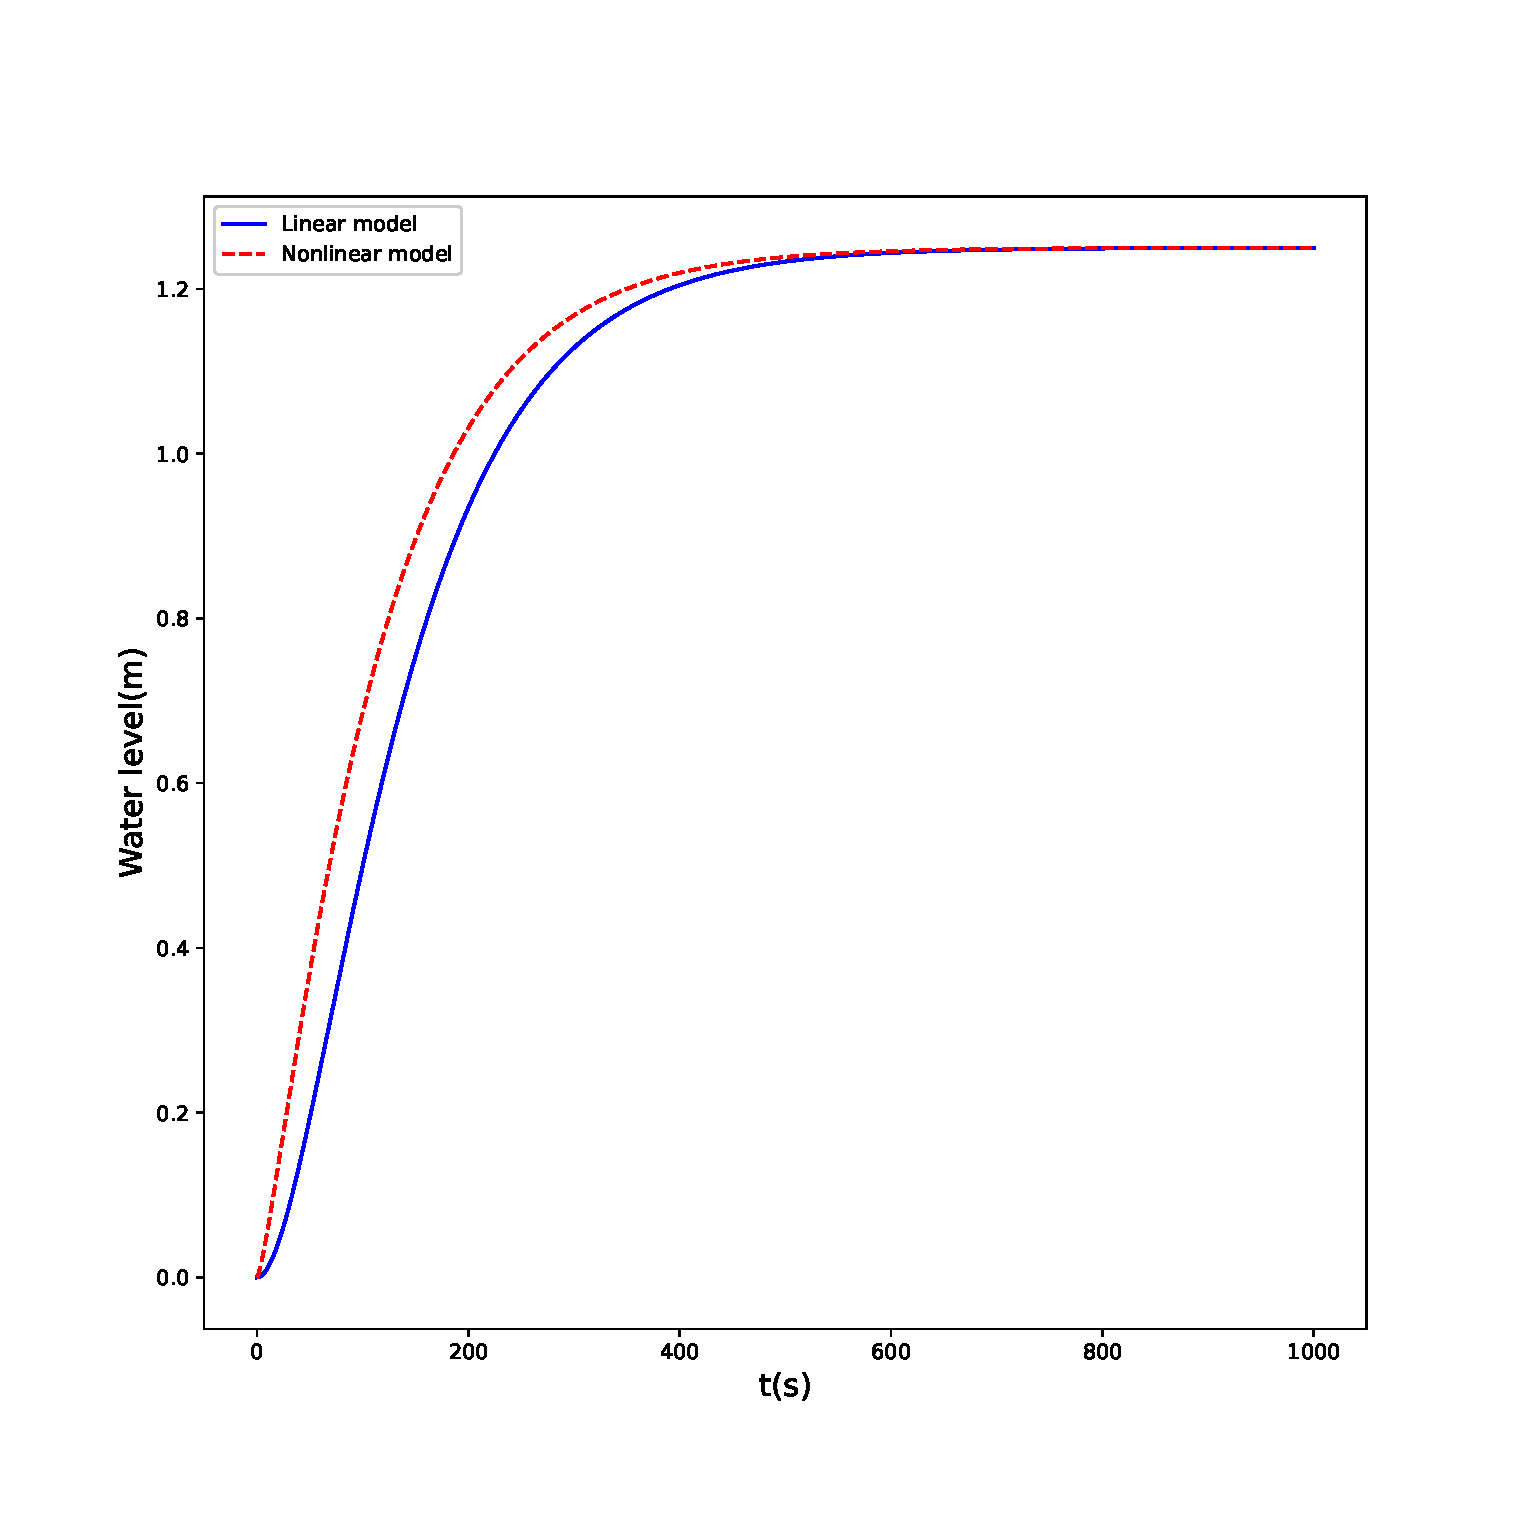
\includegraphics[width=0.4\columnwidth]{Figures/Question1/Compare.eps}
\caption{The linear model and nonlinear model step response}
\end{figure}
\par We can evaluate this model by calculating the mean square error, comparing the output of the non-linear model with the linear model.
\begin{align*}
MSE = \frac{1}{n}\sum_{i=1}^n(y_i-\bar{y}_i)^2
\end{align*}
\par The MSE of the data in the plot is 0.005118364763179614, if we modify the input magnitude and check the MSE again we get the following graph:
\begin{figure}[H]
\centering
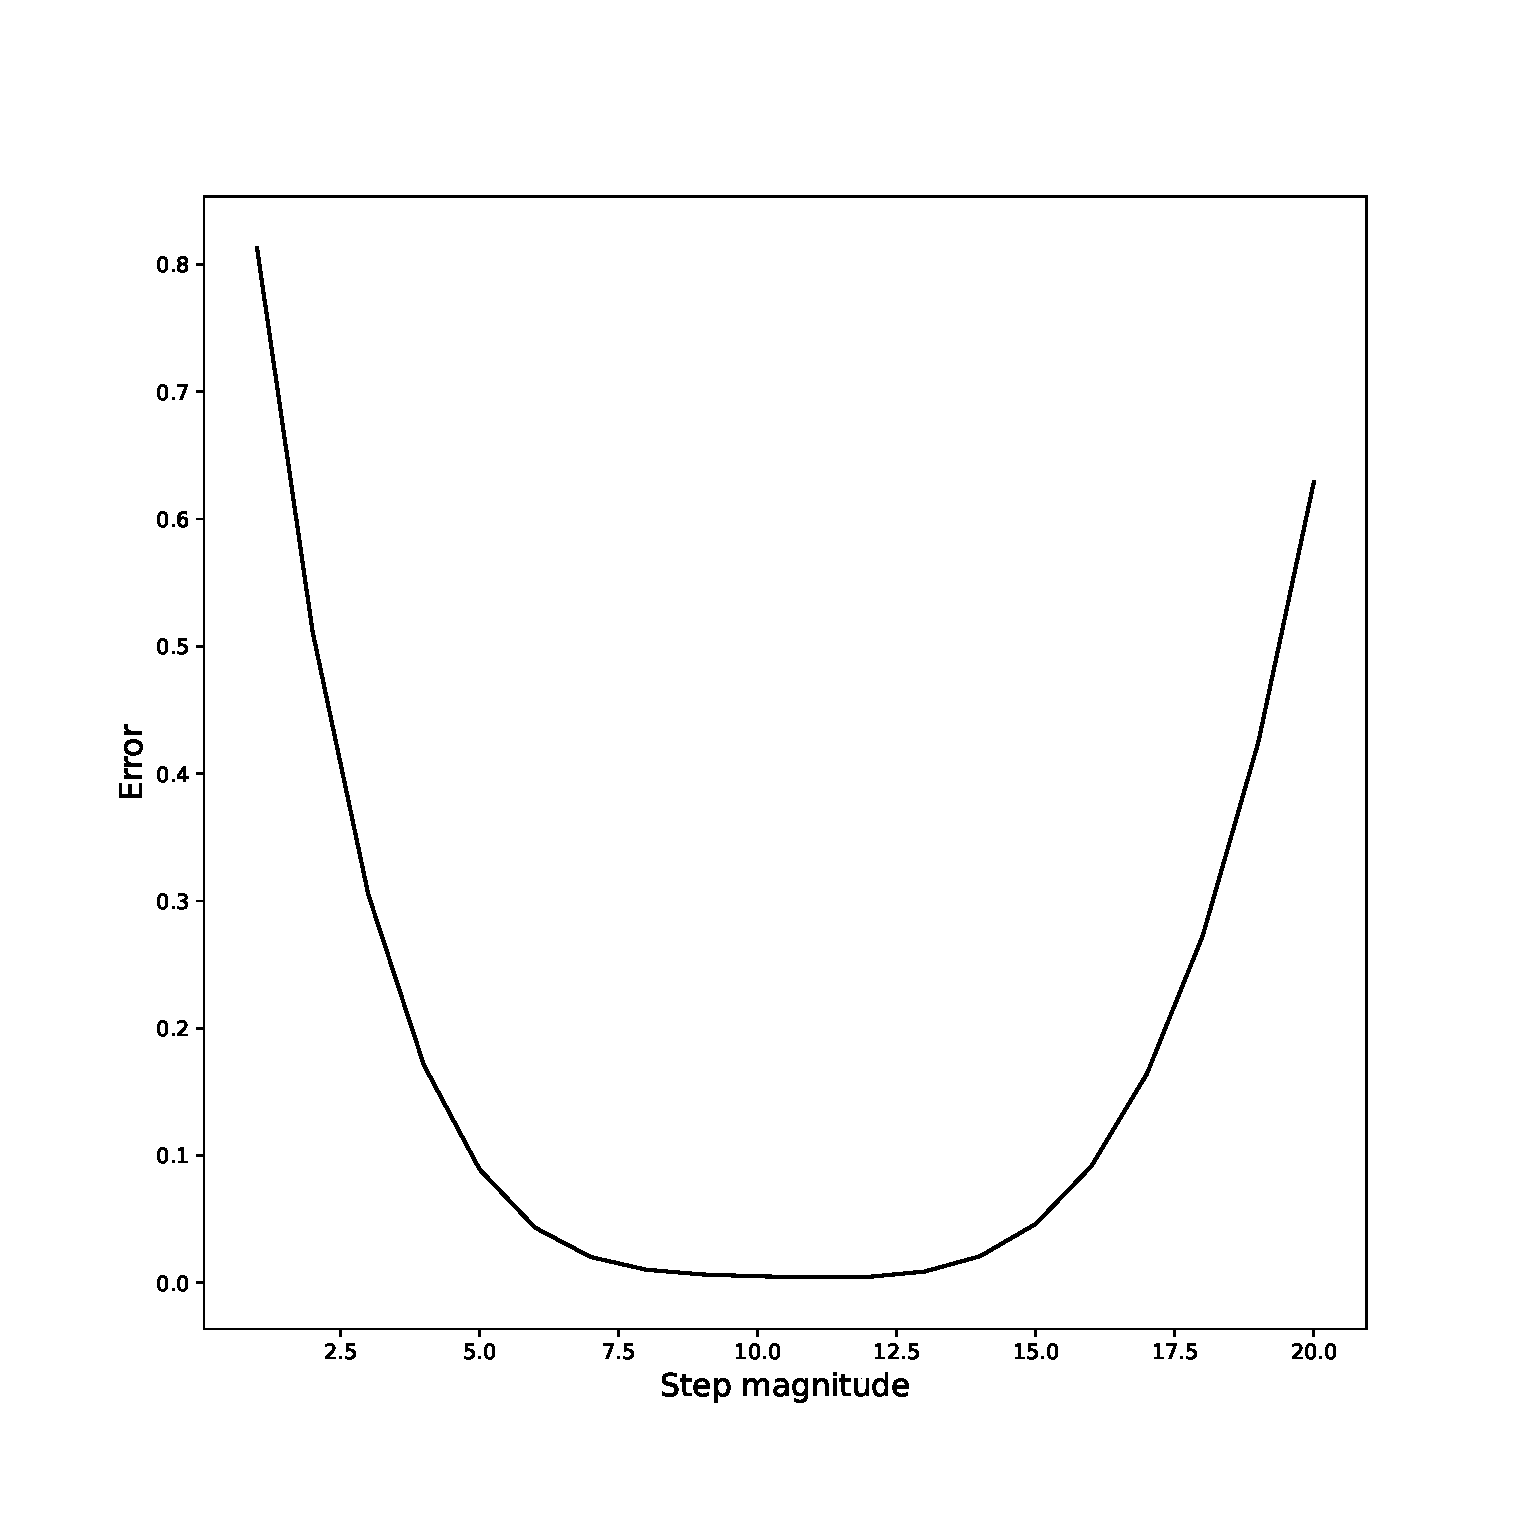
\includegraphics[width=0.4\columnwidth]{Figures/Question1/Error.eps}
\caption{The Mean square error of the output comparing the linear and nonlinear model}
\end{figure} 
\par The graph above shows that the model developed represents a good description of the system for steps with a magnitude close to 10, this is a consequence of the considerations taken in the linearization process, in it we use the input with magnitude 10, so it is expected that the model is better at his neighborhood.
\section*{Exercise 2} 
Consider the input-output model in \ref{eq:Eq9}
\begin{equation}
\cfrac{d^2y(t)}{dt^2}+4\cfrac{dy(t)}{dt}+5y(t)=\cfrac{du(t)}{dt}+5u(t)
\label{eq:Eq9}
\end{equation} 
\begin{enumerate}
\item Define the characteristic polynomial and plot the system modes.
\item Given the initial conditions in (\ref{eq:Eq6}), find the free evolution of the system in (\ref{eq:Eq5}):
\begin{equation}
y(t)\Big\vert_{t=0}=2, \quad \cfrac{dy(t)}{dt}\Big\vert_{t=0}=1
\label{eq:Eq10}
\end{equation}
\item Find the forced response of the system subject to a unit step input.
\item Plot the response $y(t)$ and comment on your results.
\end{enumerate}
\subsection*{Solution} 
\par The equation \eqref{eq:Eq9} describes a linear system because it follows the superposition principle. Based on this, the system response can be divided into a forced response and a free response. The force response does not consider the initial states of the system, it only evaluates the response to the input. The free answer does not consider the input and only considers the initial conditions. We represent as follows:
\begin{align*}
y(t) = y_0(t) + y_u(t)
\end{align*}
\par Where $y_0(t)$ represents the free output response and $y_u(t)$ is the forced output response. To find them we can apply the Laplace transform in the equation \eqref{eq:Eq9}.
\par Before find the forced and free response due to information from the question, let's present the characteristica polynomial. To find it, it's only necessary to apply the Laplace transform in the \eqref{eq:Eq9}. We find:  
\begin{align*}
s^2Y(s)+4sY(s)+5Y(s)-(sy(0)+\dot{y}{(0)}+4y(0))&= sU(s)+5U(s)
\end{align*}
We can manipulate the equation to the next:
\begin{align}
\label{eq:Eq11}
Y(s)(s^2+4s+5)&= sU(s)+5U(s)+(sy(0)+\dot{y}{(0)}+4y(0))
\end{align}
\par The characteristic polynomial is the term that multiply Y(s), it is:
\begin{align}
\label{eq:Eq12}
p(s)=s^2+4s+5
\end{align}
\par In the equation \eqref{eq:Eq11} we used the forced and free response considerations: 
\begin{itemize}
\item Considering only the step input effect:
\begin{align*}
Y_f(s)(s^2+4s+5) &=\frac{1}{s}(s+5)\\
Y_f(s) &= \frac{(s+5)}{s(s^2+4s+5)}
\end{align*}
\item Considering only the initial conditions effect:
\begin{align*}
Y_0(s)(s^2+4s+5) &= sy(0) \dot{y}(0)+4y(0)=2s+9\\
Y_0(s) &=\frac{2s+9}{(s^2+4s+5)}
\end{align*}
\end{itemize}
\par Now it's only necessary to find the inverse Laplace transform of each equation, in \ref{lst:2first} we can find the inverse Laplace computationally, the next steps going to use partial fractions way. Let's begin with the forced response. 
\par Before divide the equation of $Y_f(s)$ into partial fractions we need to find the roots of the characteristic polynomial, using some mathematical techniques approach the roots are:
\begin{align*}
s_1 = -2+i\\
s_2 = -2-i
\end{align*}
\par Then the partial fraction for the forced response is:
\begin{align}
\label{eq:Eq13}
Y_f(s) = \frac{A}{s}+\frac{K}{s+2-i}+\frac{K^*}{s+2+i}
\end{align}
\par The residues are:
\begin{align*}
	A &= \lim_{s \rightarrow 0}\frac{s+5}{s^2+4s+5}=1\\
	K &= \lim_{s \rightarrow -2+i} = \frac{(s+5)}{s(s+2+i)} =\frac{3+i}{(-2+i)(2i)}=\frac{3+i}{-(2+4i)}=\frac{-(3+i)(2-4i)}{20}=-0.5+0.5i \\
	K^*&=-0.5-0.5i
\end{align*}
\par Now applying the inverse Laplace transform:
\begin{align*}
y_f(t) = 1+(-0.5+0.5i)e^{(-2+i)t}+(-0.5-0.5i)e^{(-2-i)t}\\
\end{align*}
\par We can represent every complex number using trigonometrical representation, for example:
\begin{align}
(-0.5+0.5i)&=-0.5(1-i)=-0.5\sqrt{2}(\cos(0.785)-i\sin(0.785)\\
(-0.5-0.5i)&=-0.5(1+i)=-0.5\sqrt{2}(\cos(0.785)+i\sin(0.785)
\end{align}

\par We also can use the Euler's formula to find:
\begin{align}
e^{(-2+i)t}=e^{-2t}(\cos(t)+i\sin(t))\\
e^{(-2-i)t}=e^{-2t}(\cos(t)-i\sin(t))
\end{align}
Then we have, for $\theta =0.785$
\begin{align*}
y_f(t) &= 1-0.5\sqrt{2}e^{-2t}((\cos(t)+i\sin(t))(\cos(\theta)-i\sin(\theta))+(\cos(\theta)+i\sin(\theta))(\cos(t)-i\sin(t)))\\
y_f(t) &= 1-0.5\sqrt{2}e^{-2t}(2\cos(t)\cos(\theta)+2\sin(t)\sin(\theta))\\
y_f(t) &= 1-\sqrt{2}e^{-2t}(\cos(t-\theta))\\
y_f(t) &= 1-1.41e^{-2t}(\cos(t-0.785))
\end{align*}
\par We can plot the last equation using the code in \ref{lst:2second}. 
\begin{figure}[H]
\centering
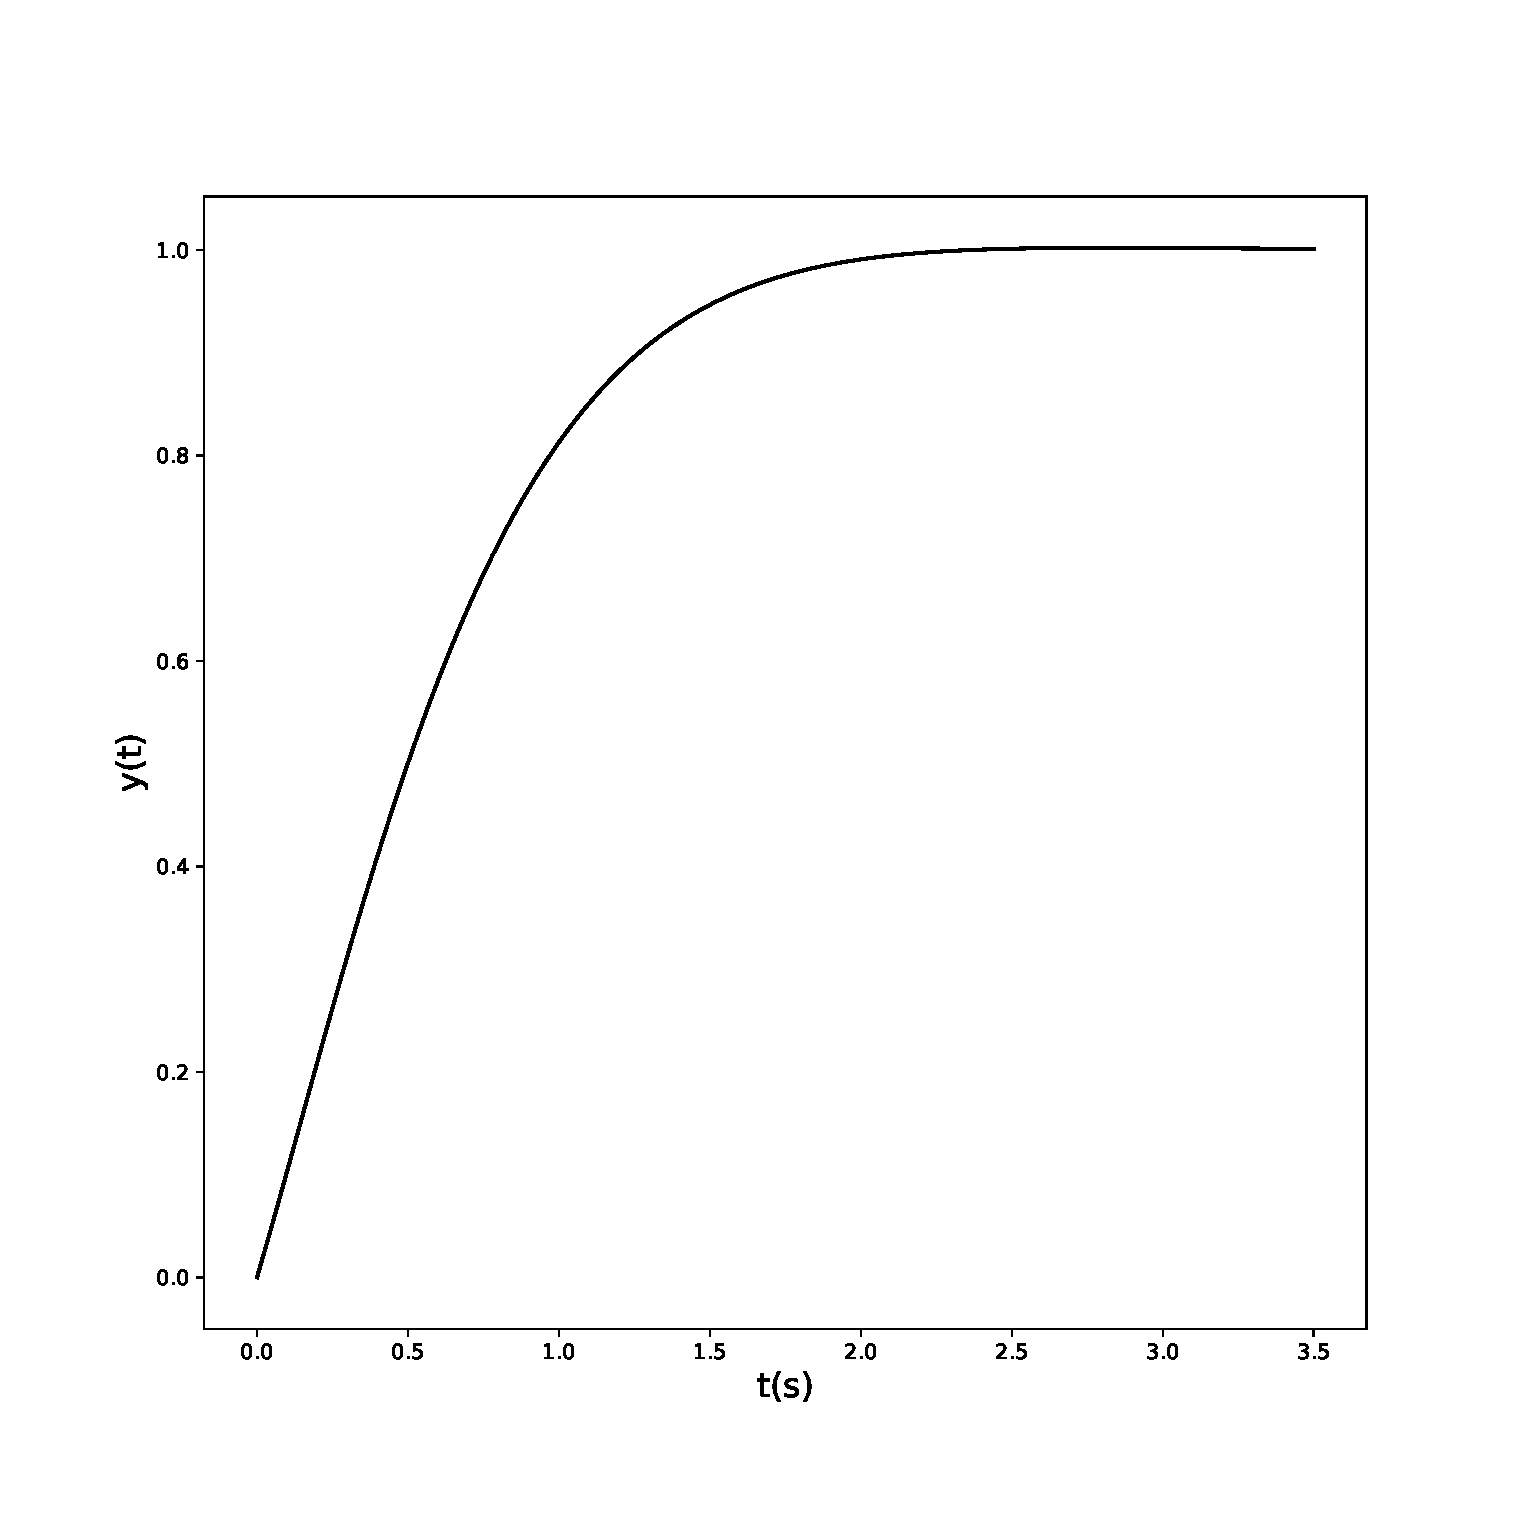
\includegraphics[width=0.4\columnwidth]{Figures/Question2/Forced.eps}
\caption{Forced response.}
\end{figure}
\par Finding the free response we need to following the same steps now for the equation:
\begin{align*}
Y_0(s) &=\frac{2s+9}{(s^2+4s+5)}
\end{align*}
\par The partial fractions are:
\begin{align*}
\frac{2s+9}{(s^2+4s+5)} &= \frac{B}{(s+2-i)}+\frac{B^*}{(s+2+i)}
\end{align*}
\par The residues are:
\begin{align*}
B &= \lim_{s\rightarrow -2+i} \frac{(2s+9)}{s+2+i}=\frac{5+2i}{2i}=1-\frac{5}{2}i\\
B^* &= 1+\frac{5}{2}i
\end{align*}
\par Then:
\begin{align*}
y_0(t) = (1-\frac{5}{2}i)e^{-2t+it}(1+\frac{5}{2}i)e^{-2t-it}
\end{align*}
\par Taking the same steps that was made for the forced response we have:
\begin{align*}
y_0(t) =5.38e^{-2t}\cos(t-1.19)
\end{align*}
\par Then the plot is:
\begin{figure}[H]
\centering
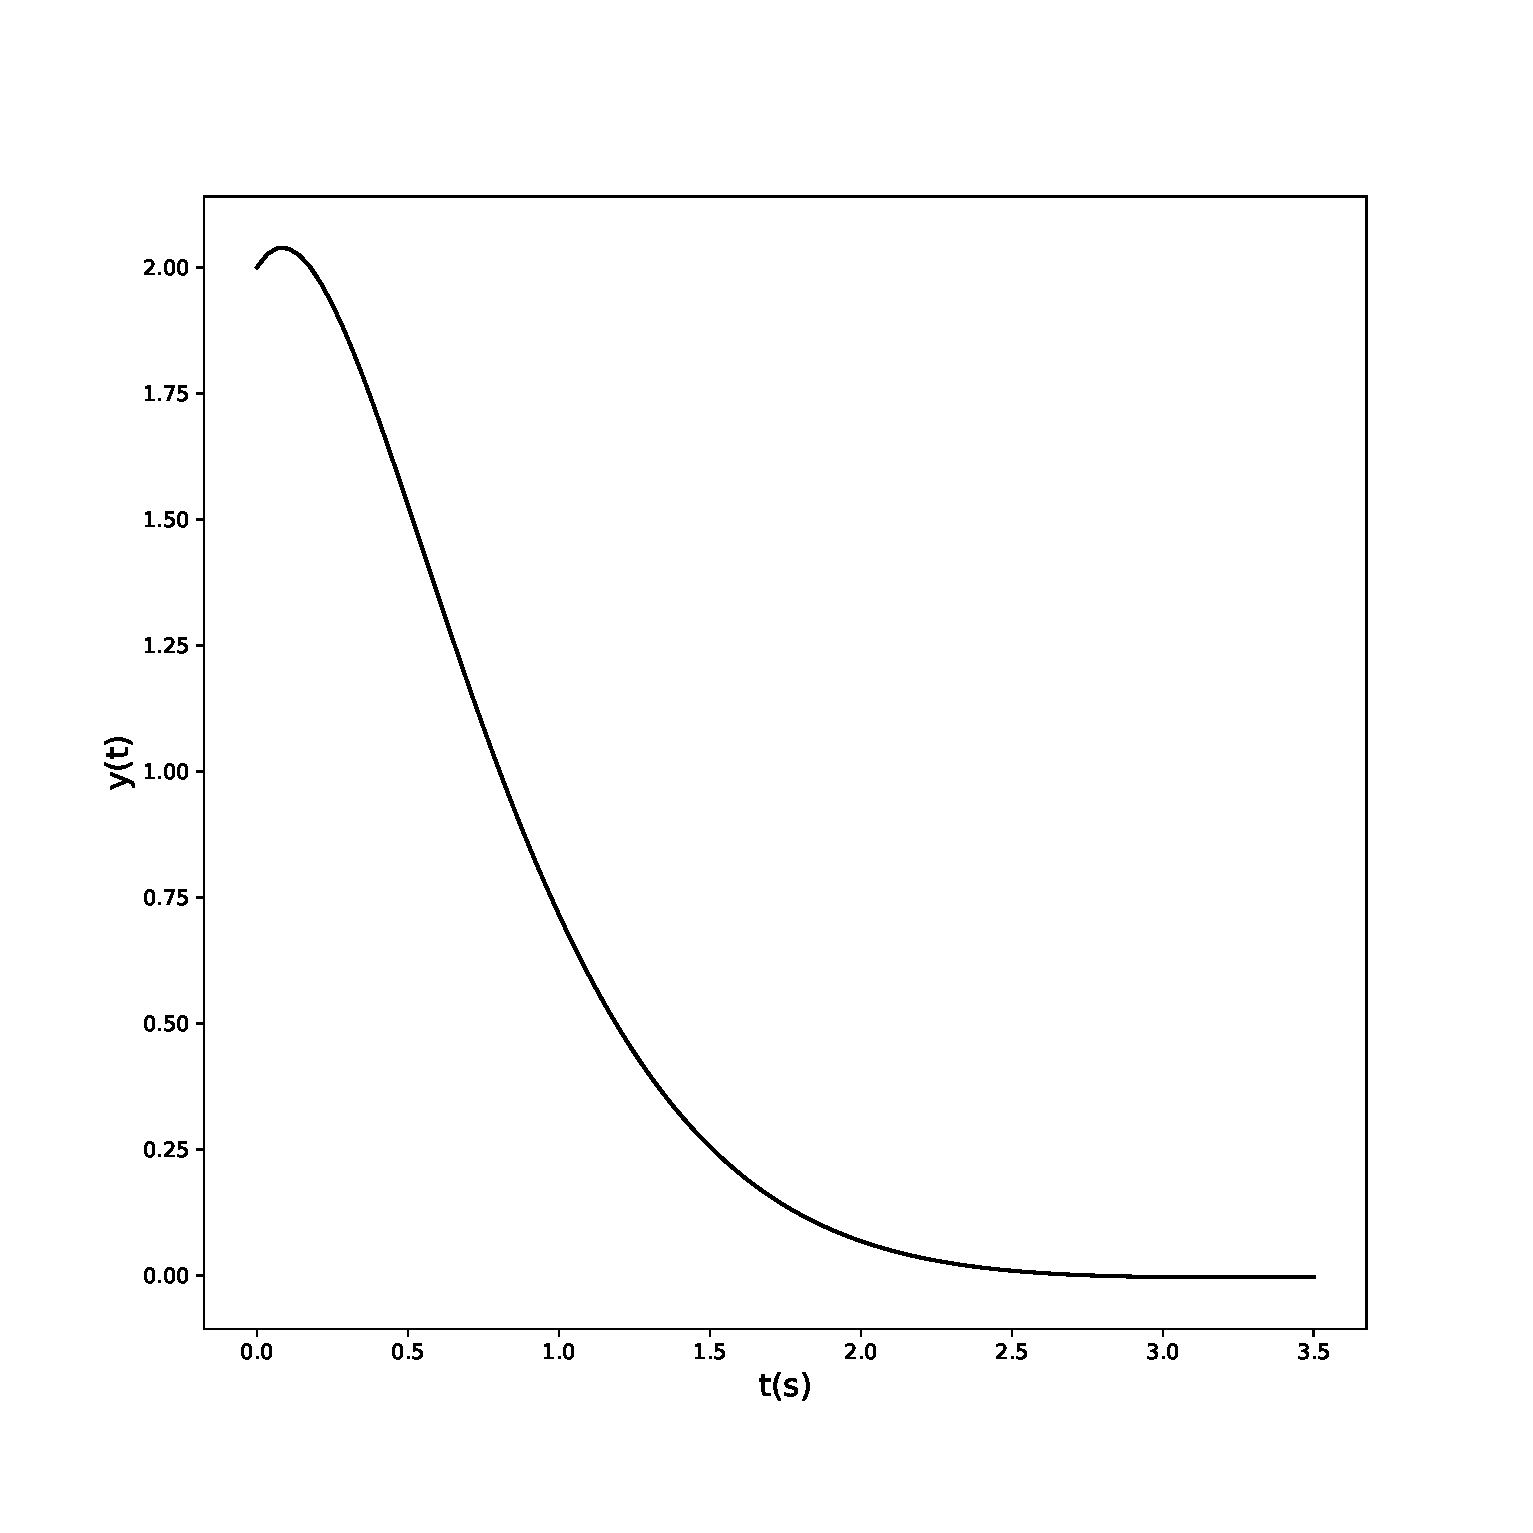
\includegraphics[width = 0.4\columnwidth]{Figures/Question2/Free.eps}
\caption{Free response.}
\end{figure}
\par In conclusion y(t) going to be:
\begin{align}
y(t) = 1+5.38e^{-2t}\cos(t-1.19)-1.41e^{-2t}(\cos(t-0.785))
\end{align}
\par Using the code in \ref{lst:2fourth} we find the system output.
\begin{figure}[H]
\centering
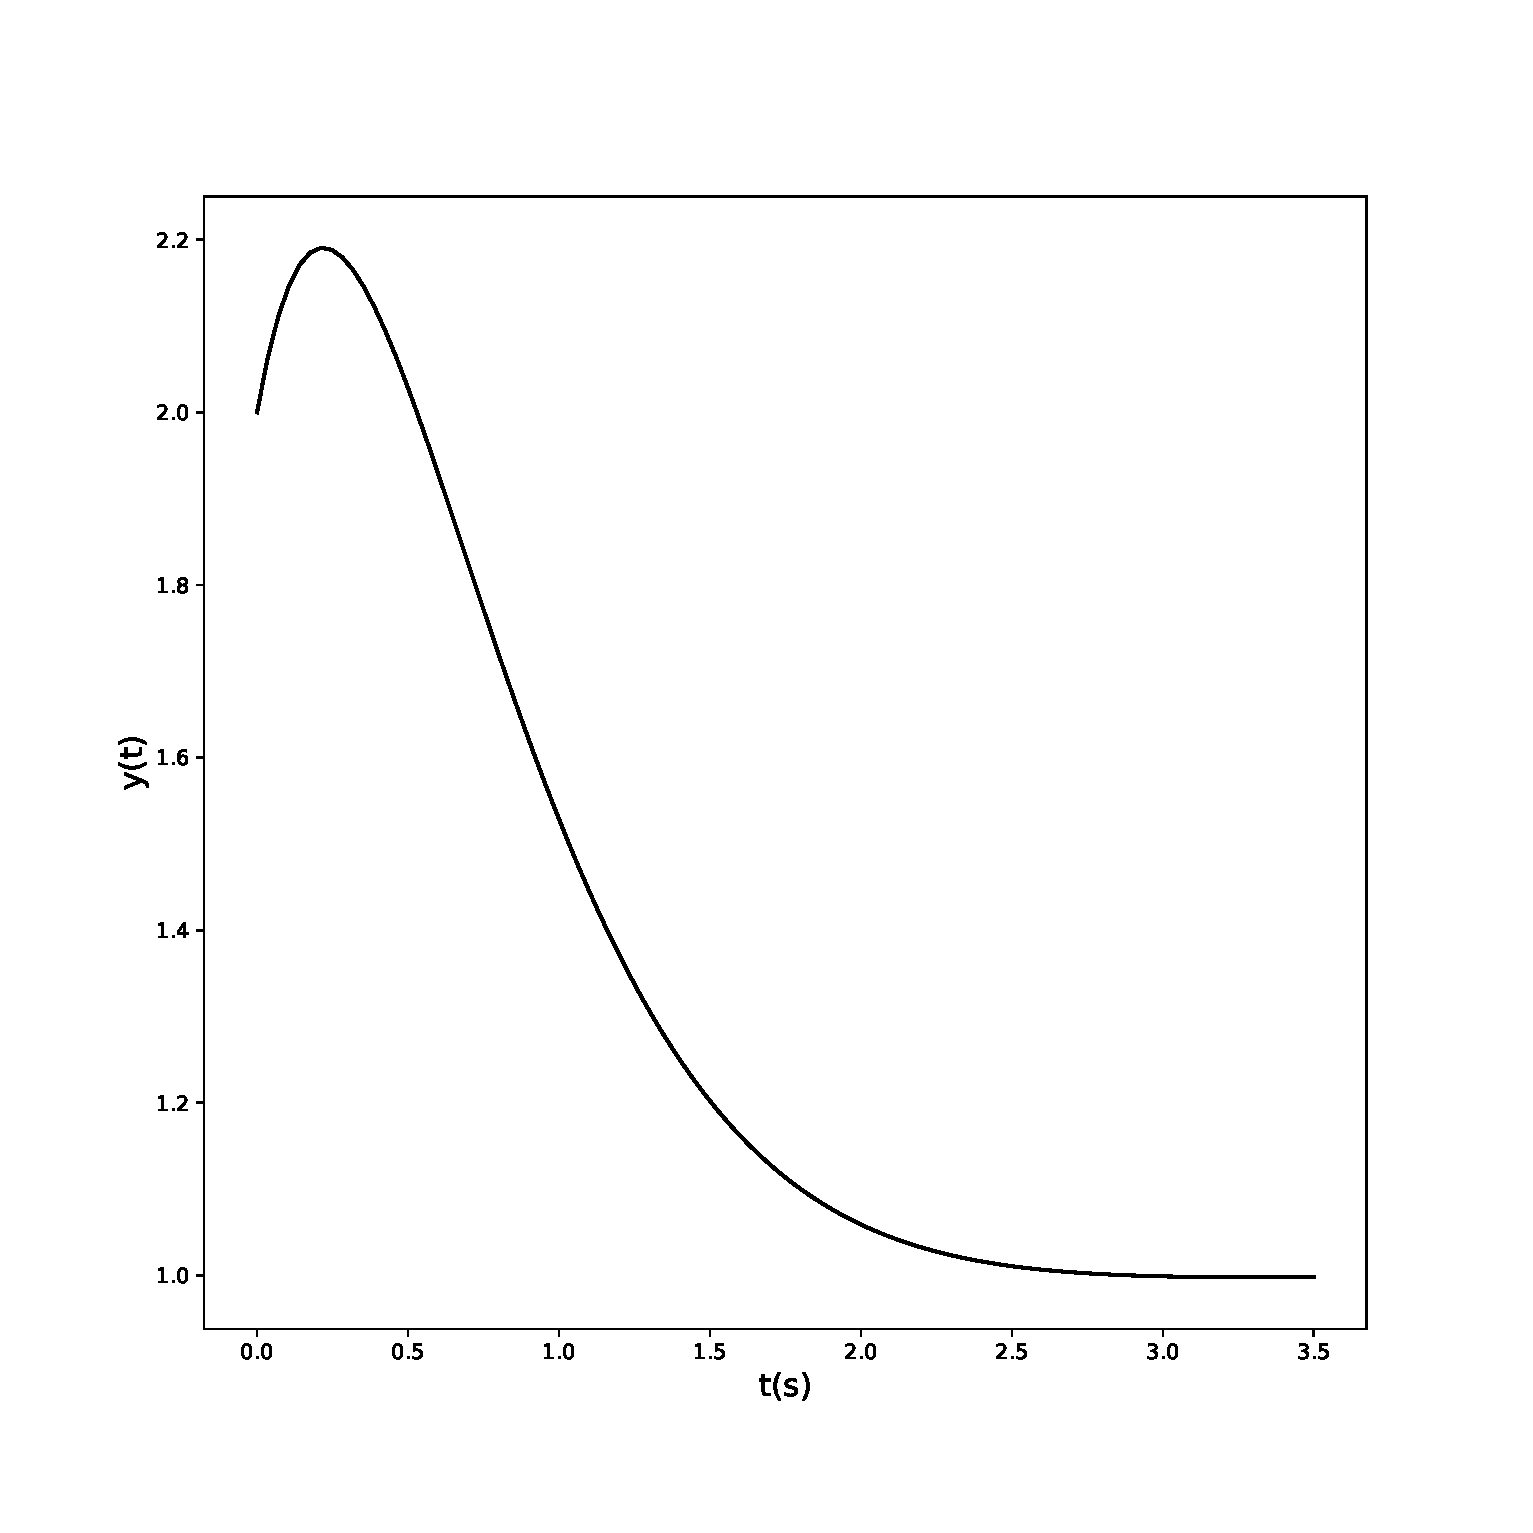
\includegraphics[width=0.4\columnwidth]{Figures/Question2/System.eps}
\caption{System response.}
\end{figure}
\par It's possible to see that the
\section*{Exercise 3}

\noindent  For a system with the transfer function in (\ref{eq:ex2}):
\begin{equation}
G(s)=\cfrac{\alpha s^2 +s+3}{s^2+2s+10}
\label{eq:ex2}
\end{equation}  

\begin{enumerate}
\item For $\alpha=1$, find and plot the unit step and impulse responses.
\item For $\alpha=[-2, \ -1, \ 0, \ 1, \ 2]$, plot and compare the unit step response.
\item Discuss how the system varies its response for the different values of $\alpha$.
\end{enumerate}

\subsection*{Solution} 
For $\alpha =1$, then we get:
\begin{align*}
G(s) = \frac{s^2+s+3}{s^2+2s+10}
\end{align*}
\par We can divide the polynomial above and get:
\begin{align}
\label{eq:Eq14}
G(s) = 1-\frac{s+7}{s^2+2s+10}
\end{align}
\par To find the response to the impulse it's only necessary applying the inverse Laplace transform of $G(s)$.
\par The inverse Laplace transform $G(s)$ can be represented as:
\begin{align*}
g(t) = \delta (t)+ \mathcal{L}^{-1}\left[\frac{s+7}{s^2+2s+10}\right]
\end{align*}
\par Where $\delta (t)$ is the impulse function. In order to calculate the other term we find the roots of the denominator, they are:
\begin{align*}
s_1 &= -1+3i\\
s_2 &= -1-3i
\end{align*}
\par Then we can define the partial fractions:
\begin{align*}
\frac{s+7}{s^2+2s+10} = \frac{A}{s+1-3i}+\frac{A^*}{s+1+3i}
\end{align*}
\par Where $A,\; A^*$ are complex conjugated. To find them we perform the following:
\begin{align*}
A &=\lim_{s\rightarrow -1+3i} \frac{s+7}{s+1+3i}=\frac{6+3i}{6i}=0.5-i\\
A^*&=0.5+i
\end{align*}
\par Then:
\begin{align*}
\mathcal{L}^{-1}\left[\frac{s+7}{s^2+2s+10}\right]= (0.5-i)e^{(-1+3i)t}+(0.5+i)e^{(-1-3i)t}
\end{align*}
\par We can represent $0.5+i$ and $0.5-i$ as:
\begin{align*}
0.5+i &= \sqrt{0.5^2+1}(\cos\theta+i\sin\theta)\\
0.5-i &= \sqrt{0.5^2+1}(\cos\theta-i\sin\theta)
\end{align*}
\par Where: $\sqrt{0.5^2+1}=1.118$ and $\theta= 1.107$.
\begin{align}
\frac{1}{2}e^{-t}\left(\left(1-2i\right) e^{3it}+ \left(1+2i\right) e^{-3it}\right)=\sqrt{5}e^{-t}\cos(3t-1.107)
\end{align}
\par Consequently the impulse response is:
\begin{align}
g(t) = \delta(t) -\sqrt{5}e^{-t}\cos\left(3t-1.107\right)
\end{align}
\par Using the code in \ref{lst:3second} we can check the answer. We can plot the impulse response using the code in \ref{lst:3third}.
\begin{figure}[H]
\centering
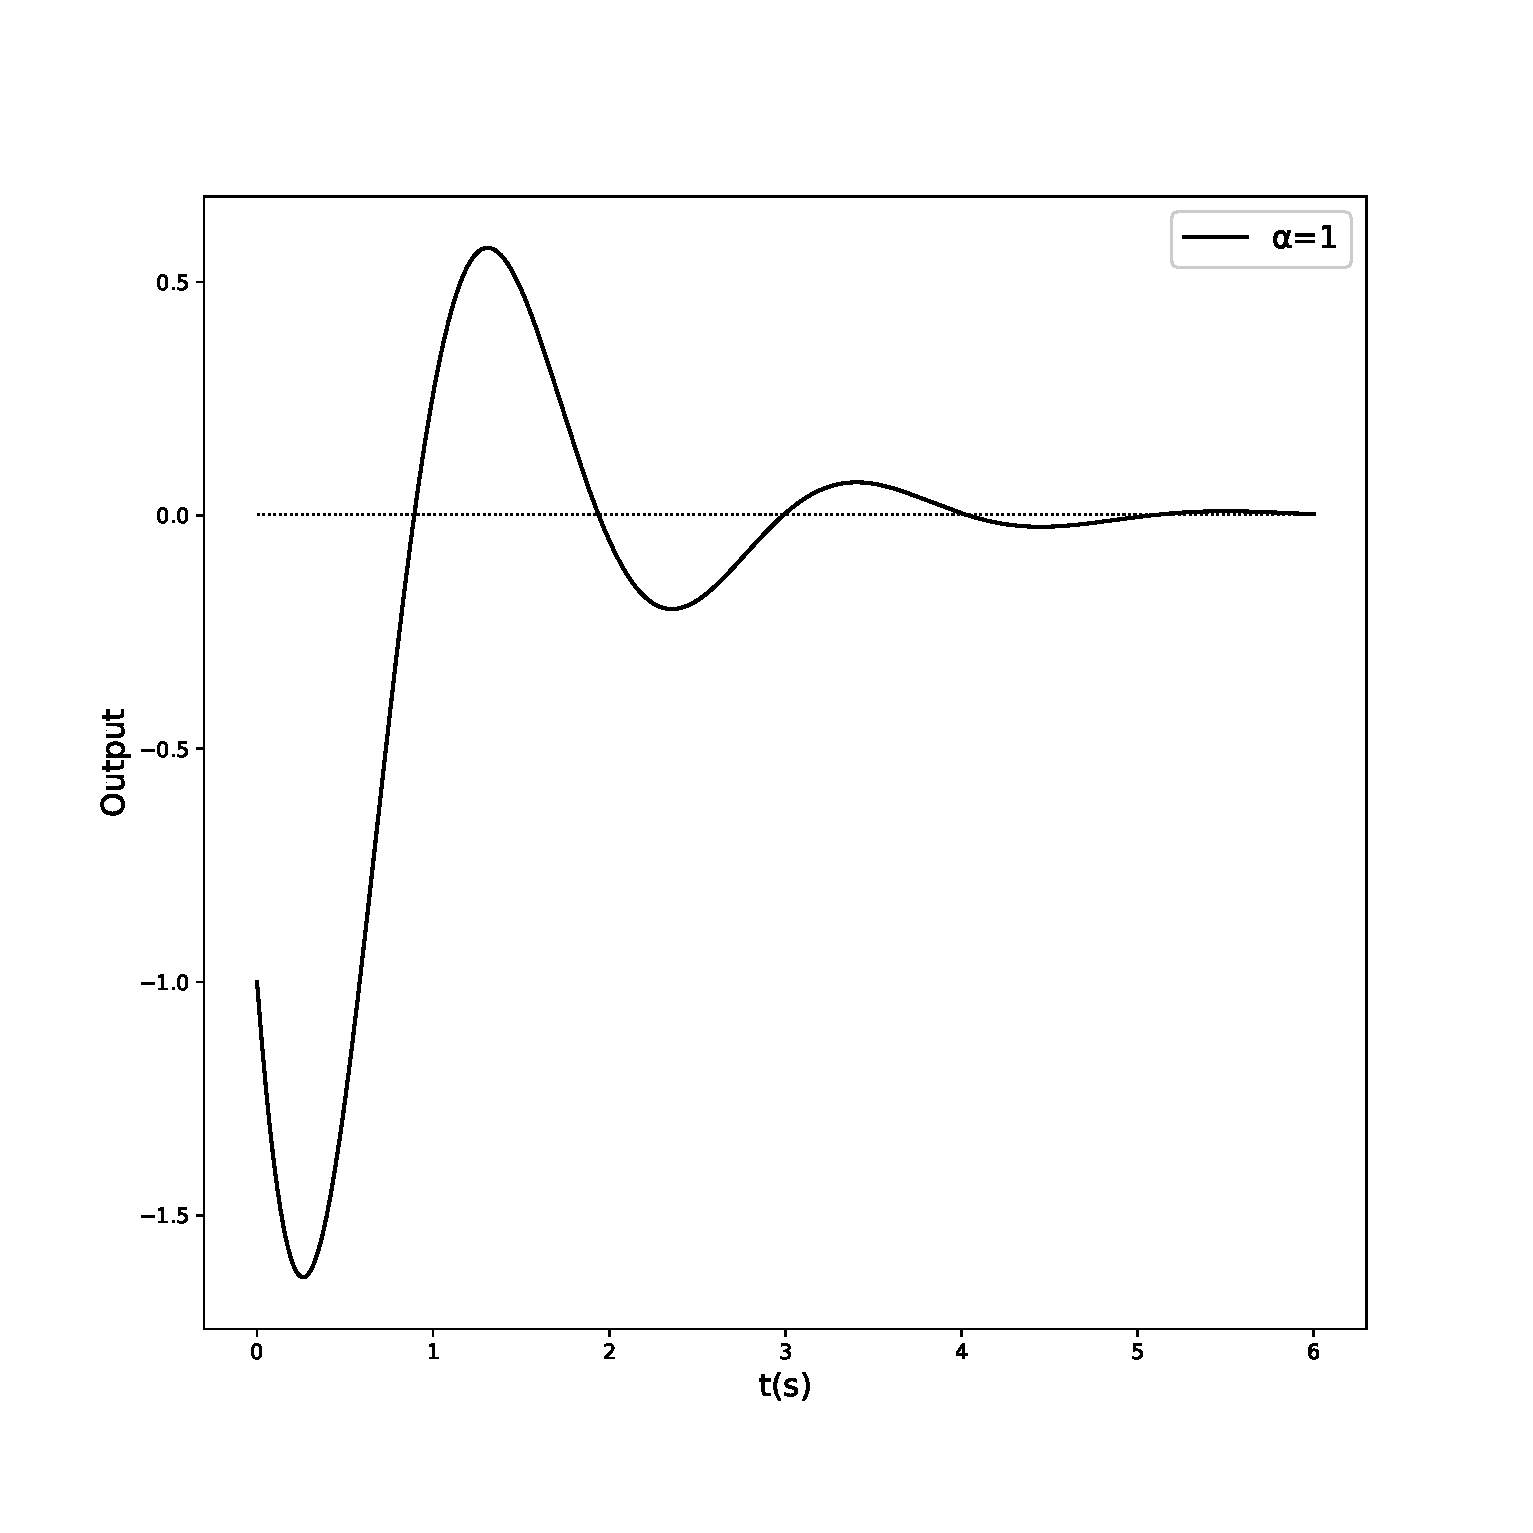
\includegraphics[width=0.4\columnwidth]{Figures/Question3/3impulseResponse.eps}
\caption{This is the impulse response when $\alpha$ =1.}
\end{figure}
\par To find the response for the step then we need to multiply G(s) by the Laplace transform of the step, $\frac{1}{s}$, then:
\begin{align}
\label{eq:Eq15}
Y(s) = \frac{1}{s}-\frac{1}{s}\frac{s+7}{(s^2+2s+10)}
\end{align}
\par The inverse Laplace transform can be represented as follow:
\begin{align*}
y(t) = 1- \mathcal{L}^{-1}\left[\frac{s+7}{s(s^2+2s+10)}\right]
\end{align*}
\par Now, lets show the partial fractions for the second term:
\begin{align*}
\left[\frac{s+7}{s(s^2+2s+10)}\right] = \frac{B}{s}+\frac{K}{s+1-3i}+\frac{K^*}{s+1+3i} 
\end{align*}
\par Calculating the residues:
\begin{align*}
B &= \lim_{s \rightarrow 0}\frac{s+7}{(s^2+2s+10)}=0.7\\
K &= \lim_{s \rightarrow -1+3i} = \frac{6+3i}{6i(-1+3i)}=-0.35-0.05i\\
K^*&=-0.35+0.05i
\end{align*}
\par So we can represent the step response as:
\begin{align}
y(t)= 0.3+(0.35+0.05i)e^{(-1+3i)t}+(0.35-0.05i)e^{(-1-3i)t}
\end{align}
\par Set in the trigonometrical representation we have:
\begin{align}
y(t) = 0.3+0.7e^{-t}\cos(3t+0.142)
\end{align}
\par Using the code in \ref{lst:3third} we can check the inverse Laplace transform and using \ref{lst:3first} we get the plot for the step response.
\begin{figure}[H]
\centering
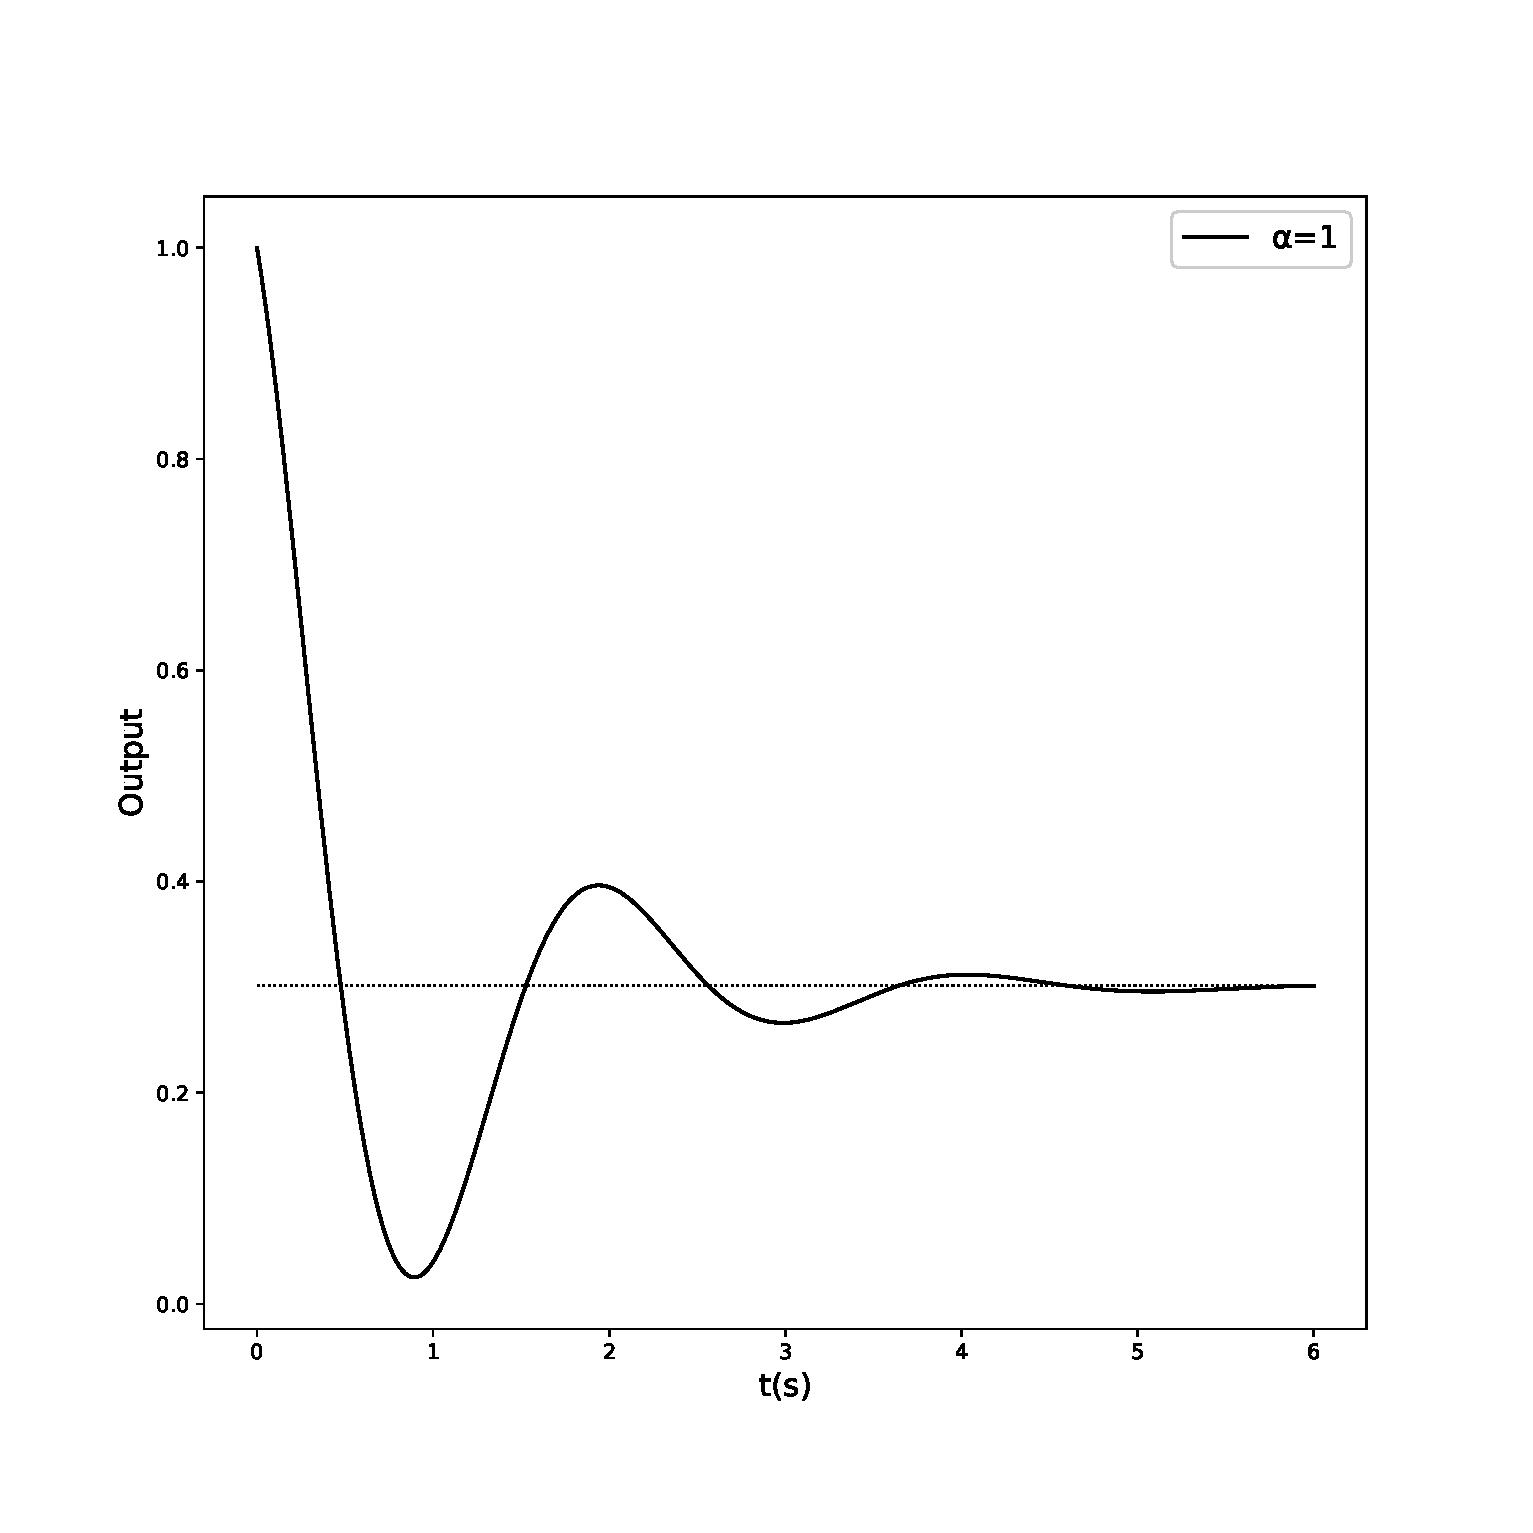
\includegraphics[width=0.5\textwidth]{Figures/Question3/3stepresponse.eps}
\caption{This is the step response when $\alpha$ =1.}
\end{figure}
\par Using the code in \ref{lst:3fifith} we can find the step response for different values of $\alpha$:
\begin{figure}[H]
\centering
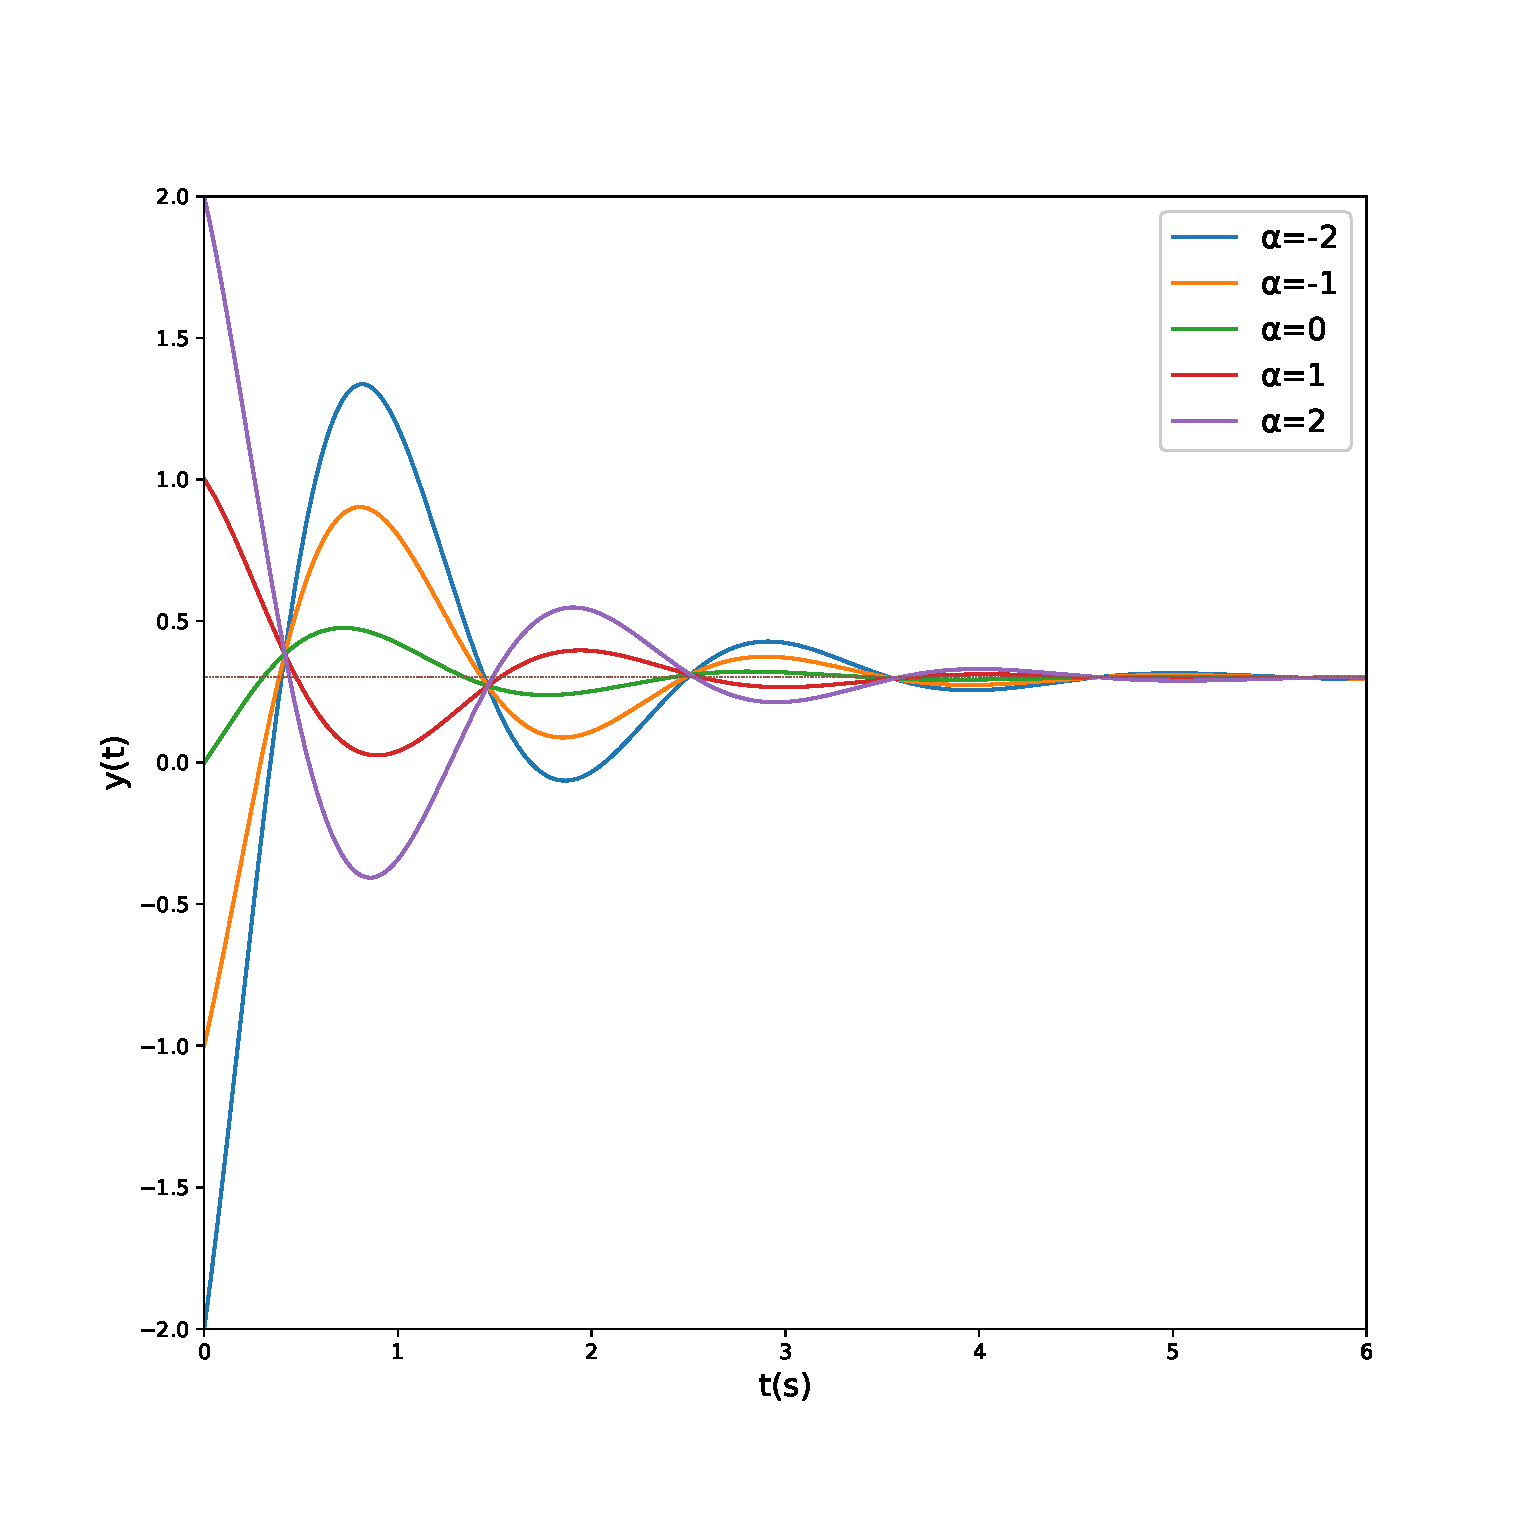
\includegraphics[width=0.4\columnwidth]{Figures/Question3/difalfa.eps}
\caption{Step response for different values of $\alpha$}
\end{figure}
\par The modification of the value of alpha, modifies how the system varies it's input comparing to the steady state value, the overshoot. Also $\alpha$ modifies the initial condition value of y(t).  
\section*{Exercise 4} 
Given the state-space model in (\ref{eq:Eq10}): \vskip-0.4cm
\begin{align}
\begin{cases}
\begin{bmatrix}
\dot{x}_1(t)\\
\dot{x}_2(t)
\end{bmatrix}
& =
\begin{bmatrix}
0 & 1\\
-4 & -5 
\end{bmatrix}
\begin{bmatrix}
{x}_1(t)\\
{x}_2(t)
\end{bmatrix}
+
\begin{bmatrix}
\ 0 \ \\
\ \cfrac{1}{4}\ 
\end{bmatrix}
u(t) \\
y(t) & =
\begin{bmatrix}
13 & 9
\end{bmatrix}
\begin{bmatrix}
{x}_1(t)\\
{x}_2(t)
\end{bmatrix}
\end{cases}
\label{eq:Eq16}
\end{align}

\begin{enumerate}
\item Find a the corresponding transfer function.
\item Find an input-output model equivalent to the state-space model. 
\item Find the state and output forced evolution as response of the input $ u(t)=e^{-t}$.
\end{enumerate}

\subsection*{Solution} 
\par Let's find the transfer function for a state space equation, first for the state space model we have this two equations:
\begin{align*}
\begin{cases}
\dot{x}(t)=Ax(t)+Bu(t)\\
y(t)=Cx(t)+Du(t)
\end{cases}
\end{align*}
\par The first equation is called the state equation and the second is the output equation. Considering the initial condition equal to zero and applying the Laplace transform to the state equation:
\begin{align*}
sX(s) &=AX(s)+BU(s)\\
X(s)(sI-A)&=BU(s)\\
X(s) &= (sI-A)^{-1}BU(s)
\end{align*}
\par Also applying the Laplace transform in the output equation and replacing the $X(s)$ value:
\begin{align*}
Y(s)= C(sI-A)^{-1}BU(s)+ DU(s)
\end{align*} 
\par In the equation \eqref{eq:Eq16} D is a null matrix, then the transfer function will going to be:
\begin{align}
\frac{Y(s)}{U(s)}=C(sI-A)^{-1}B
\end{align}
\par To calculate the transfer function we used the code in \ref{lst:4first}, and it result in:
\begin{align}
\label{eq:Eq17}
\frac{Y(s)}{U(s)}=\frac{2.25 s + 3.25}{s^2 + 5 s + 4}
\end{align}
\par To find the input-output description, we only need to manipulate the equation \eqref{eq:Eq9} as:
\begin{align*}
Y(s)(s^2+5s+4)=U(s)(2.25s+3.25)
\end{align*}
\par Now applying the inverse Laplace transform in both sides:
\begin{align}
\ddot{y}(t)+5\dot{y}(t)+4y(t) = 2.25\dot{u}(t)+3.25u(t)
\end{align}
\par To find the state forced response of the system we use the equations for each space in time:
\begin{align*}
\dot{x_1}(t) &= x_2(t)\\
\dot{x_2}(t) &= -4x_1(t)-5x_2(t)+\frac{1}{4}u(t)
\end{align*}
\par For a $u(t) = e^{-t}$ and applying a Laplace transform:
\begin{align*}
sX_1(s) &= X_2(s)\\
sX_2(s) &= -4X_1(s)-5X_2(t) +\frac{1}{4(s+1)}
\end{align*}
\par Finding $X_1(s)$:
\begin{align*}
X_1(s)(s^2+5s+4)&=\frac{1}{4(s+1)}\\
X_1(s)&=\frac{1}{4(s+1)(s^2+5s+4)}
\end{align*}
\par Now let's apply the inverse Laplace transform to find $x_1(t)$. First let's find the partial fraction for to represent $X_1(s)$. The roots of the numerator polynomial are:
\begin{align*}
s_1 = -1\\
s_2 = -4
\end{align*}
\par The $X_1(s)$ is:
\begin{align*}
X_1(s) = \frac{1}{4(s+4)(s+1)^2}=\frac{A}{(s+4)}+\frac{B}{(s+1)}+\frac{C}{(s+1)^2}
\end{align*}
\par The residues are:
\begin{align*}
A &= \lim_{s\rightarrow -4} \frac{1}{4(s+1)^2}=\frac{1}{36}=0.028\\
C &= \lim_{s\rightarrow -1} \frac{1}{4(s+4)}= \frac{1}{12}= 0.083\\
B &= \lim_{s\rightarrow -1} \frac{d\frac{1}{4(s+4)}}{ds}=-0.028
\end{align*}
\par Then:
\begin{align}
x_1(t)= 0.028e^{-4t}+0.083te^{-t}-0.028e^{-t}
\end{align}
\par $x_2$ is derivative of $x_1(t)$, then:
\begin{align}
x_2(t)= 0.028e^{-t}-0.083te^{-t}-0.112te^{-4t}
\end{align}
\par The $y(t)$ value is:
\begin{align}
y(t) = 13x_1(t) + 9x_2(t)=(1.833t - 0.611)e^{-t} + 0.611e^{-4t}
\end{align}
\par The plot of the two states and the output are:
\begin{figure}[ht]
\begin{subfigure}{.5\textwidth}
  \centering
  % include first image
  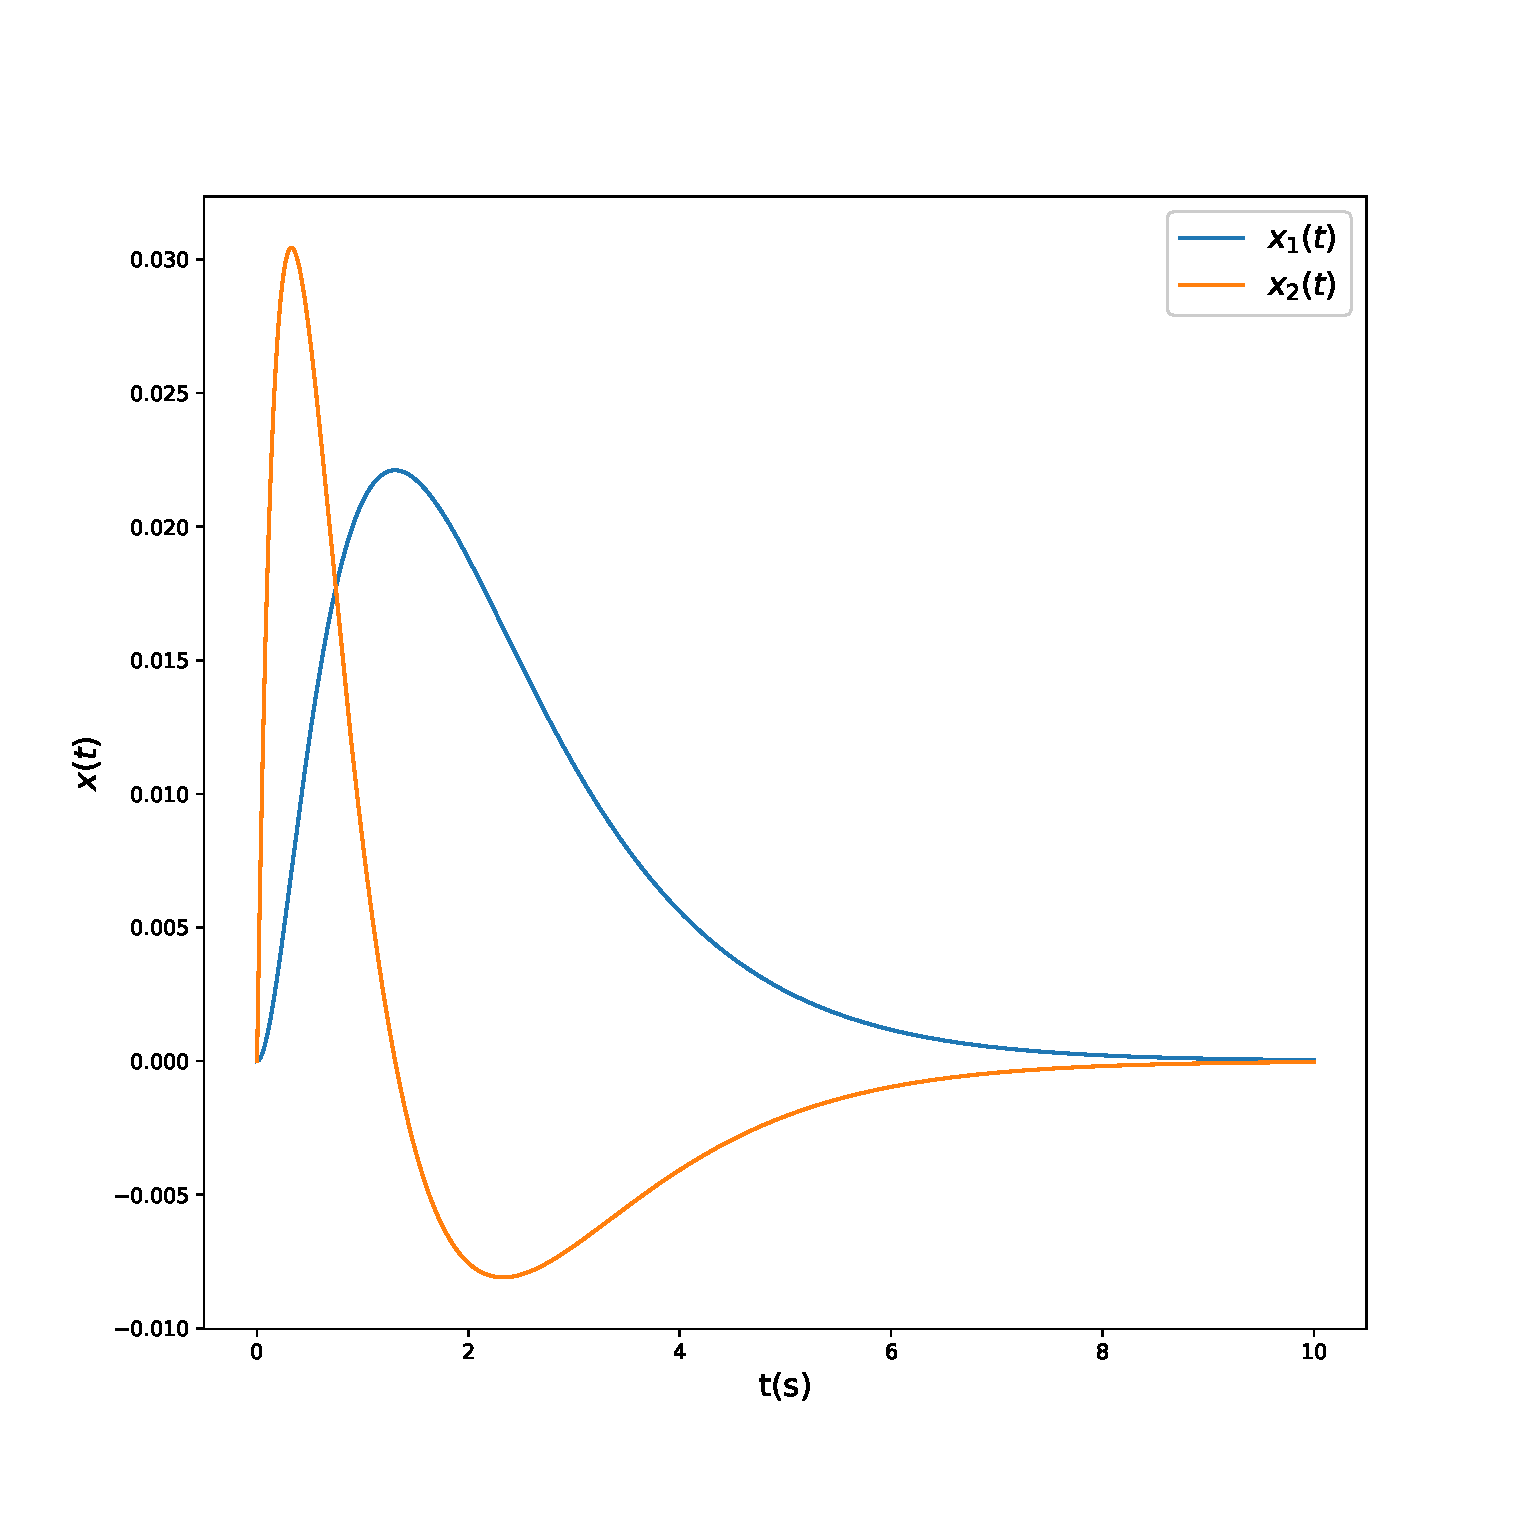
\includegraphics[width=.8\linewidth]{Figures/Question4/4stateplot.eps}  
  \caption{This the state variation in time} 
  \label{fig:sub-first}
\end{subfigure}
\begin{subfigure}{.5\textwidth}
  \centering
  % include second image
  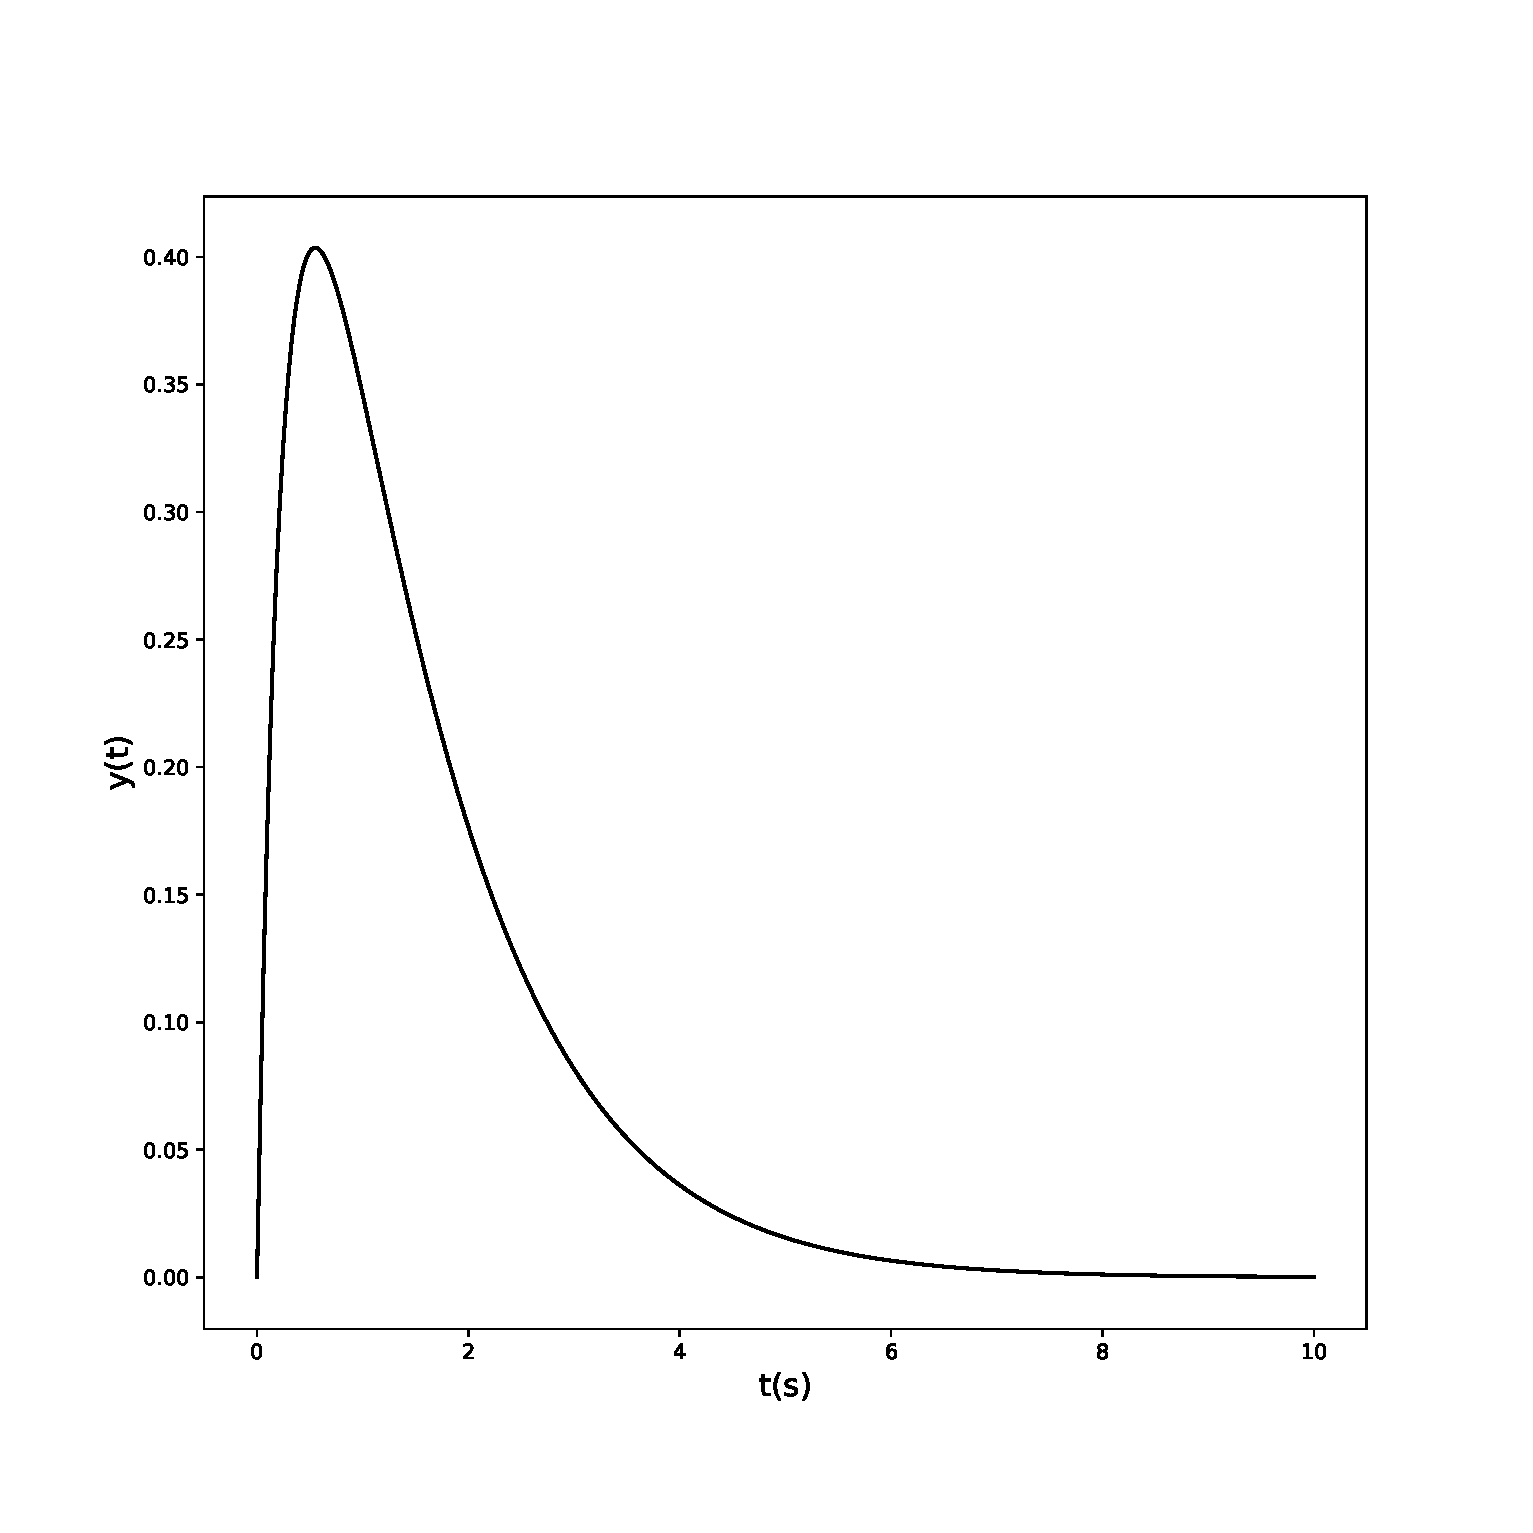
\includegraphics[width=.8\linewidth]{Figures/Question4/4output.eps} 
\caption{This is the output response in time}  
	\label{fig:sub-second}
\end{subfigure}
\caption{System output and state variation in time}
\end{figure}
\section*{Exercise 5}

\noindent Find the inverse Laplace transform by hand calculations and verify your results using the Symbolic toolbox for the following functions: 
\begin{enumerate}
\item $F_1(s)=\cfrac{s-10}{(s+2)(s+5)}$ 
\item $F_2(s)=\cfrac{100}{(s+1)(s^2+4s+13)}$
\item $F_3(s)=\cfrac{s+18}{s(s+3)^2}$ 
\end{enumerate}

{\large \sc \noindent \sc Solution} 					\\ 

\subsection*{First Item}
\par The item already informed the roots of the denominator. So the partial fractions representation of $F_1(s)$ is:
\begin{align}
F_1(s)=\frac{s-10}{(s+2)(s+5)}=\frac{A}{(s+2)}+\frac{B}{(s+5)}
\end{align}
\par The residues of the partial fractions are:
\begin{align*}
A &= \lim_{s\rightarrow -2} \frac{s-10}{s+5}=-4\\
B &= \lim_{s\rightarrow -5} \frac{s-10}{s+2}=5
\end{align*}
\par Then the inverse Laplace transform is:
\begin{align}
f(t)= -4e^{-2t}+5e^{-5t}
\end{align}
\par We can check this value using the code in \ref{lst:5first}.
\vspace{1mm}
\subsection*{Second Item}
\par The item gives just one root of the denominator, $s_1=1$, consequently we need to find the roots of the polynomial before to find the partial fraction representation. Then we can calculate the discriminant:
\begin{align}
\Delta = 16-52=-36
\end{align}
\par Consequently the roots of the polynomial are:
\begin{align*}
s_2 &=\frac{-4+\sqrt{-36}}{2} = \frac{-4 + 6i}{2}=-2 +3i\\
s_3 &=\frac{-4-\sqrt{-36}}{2} =\frac{-4-6i}{2}= -2-3i
\end{align*}
\par So the partial fractions are:
\begin{align*}
\frac{100}{(s+1)(s^2+4s+13)}=\frac{100}{(s+1)(s+2-3i)(s+2+3i)}=\frac{A}{s+1}+\frac{B}{s+2-3i}+\frac{B^*}{s+2+3i}
\end{align*}
\vspace{1mm}
\par We can prove that $B$ and $B^*$ are complex conjugate, then we only need to calculate one of them to find the other. Based on this we calculate the residues as: 
\begin{align*}
A  &= \lim_{s \rightarrow -1} \frac{100}{(s+2-3i)(s+2+3i)}=\frac{100}{(1-3i)(1+3i)}=\frac{100}{10}=10\\
B  &= \lim_{s \rightarrow -2+3i} \frac{100}{(s+1)(s+2+3i)} = \frac{100}{(-1+3i)(6i)}=\frac{100}{-(6i+18)}=\frac{-100(18-6i)}{360}=-5+1.67i\\
B^*&= -5 -1.67i
\end{align*}
\par Now the inverse transform is:
\begin{align*}
f_2(t)&=10e^{-t}+(-5+1.67i)e^{(-2+3i)t}+(-5-1.67i)e^{(-2-3i)t}\\
f_2(t)&=10e^{-t}-((5-1.67i)e^{(-2+3i)t}+(5+1.67i)e^{(-2-3i)t} 
\end{align*}
\par We represent $(5+1.67i)$ and $5-1.67i$ as:
\begin{align*}
5+1.67i &= \sqrt{5^2+1.67^2}(\cos\theta + i \sin\theta)\\
5-1.67i &= \sqrt{5^2+1.67^2}(\cos\theta-i\sin\theta)
\end{align*}
\par Where $\theta=arctg(1.67/5)=0.322$ and $\sqrt{5^2+1.67^2}=5.27$.\\
\par Also, we can use Euler's formula:
\begin{align*}
e^{(-2+3i)t}=e^{-2t}(\cos(3t)+i\sin(3t))\\
e^{(-2-3i)t}=e^{-2t}(\cos(3t)-i\sin(3t))
\end{align*}
\par Then:
\begin{align*}
f_2(t) &= 10e^{-t}-5.27e^{-2t}((\cos\theta-i\sin\theta)(\cos(3t)+i\sin(3t))+(\cos\theta+i\sin\theta)(\cos(3t)-i\sin(3t))\\
f_2(t) &= 10e^{-t}-5.27e^{-2t}(2\cos\theta\cos(3t)+2\sin\theta\sin(3t))\\
f_2(t) &= 10e^{-t}-10.54e^{-2t}(\cos(3t-\theta))
\end{align*}
\par In conclusion:
\begin{align}
f_2(t)=10e^{-t}-10.54(e^{-2t}(\cos(3t-0.32)))
\end{align}
\par We can check the same answer using the code in \ref{lst:5second}.
\subsection*{Third item}
The item already informed the roots of the denominator. So the partial fractions representation of $F_3(s)$ is:
\begin{align*}
\frac{s+18}{s(s+3)^2}=\frac{A}{s}+\frac{B}{(s+3)}+\frac{C}{(s+3)^2}
\end{align*}
\par The residues are:
\begin{align*}
A &= \lim_{s \rightarrow 0}\frac{s+18}{(s+3)^2}=\frac{18}{9}=2\\
C &= \lim_{s \rightarrow -3}\frac{s+18}{s}=\frac{15}{-3}=-5\\
B &= \lim_{s \rightarrow -3}\frac{d\frac{(s+18)}{s}}{ds}=\lim_{s \rightarrow -3}\frac{-18}{s^2}=-2
\end{align*}
\par In conclusion :
\begin{align}
f(t) = 2-2e^{-3t}-5e^{-3t}t
\end{align}
\par We can check the answer using the code in \ref{lst:5third}
\newpage
\section*{Appendix}
\appendix 
\begin{itemize}
\item Obs 1: I created a online Notebook with the code for solving each question of this homework
: \href{https://colab.research.google.com/drive/1j09ifwj77xrI9G4FtcCSJtw4kdnd3njG}{Notebook with the answer}. The notebook is a living representation of the next section source code.
\end{itemize}
\section{Source code for exercise 1}
\begin{lstlisting}[caption={System Nonlinear function simulation}\label{lst:1first}]
def nonlineartank(x,t,params):
  [x1,x2]=x
  [A1,A2,u,mi1,mi2,mi3,g] = params
  f1 = (1/A1)*(u-2*mi1*((2*g*x1)**(0.5)))
  f2 = (1/A2)*((mi1*((2*g*x1)**0.5))-(mi2*((2*g*x2)**0.5)))
  dx =[f1,f2]
  return dx
from scipy.integrate import odeint
T=np.arange(0,1000,0.001)
A1 =200
A2 =200
mi1 = 1
mi2 = 1
mi3 = 1
g = 10
u = 1
yode=odeint(nonlineartank,[0,0],T,args=([A1,A2,u,mi1,mi2,mi3,g],))
plt.plot(T,yode[:,1],'k')
plt.xlabel('t(s)',fontsize=15)
plt.ylabel('Water level (m)',fontsize=15)
plt.rcParams["figure.figsize"] = (10,10)
plt.savefig('Question1Nonlinear.eps', format='eps')
\end{lstlisting}
\begin{lstlisting}[caption={System linear simulation function}\label{lst:1second}]
import control.matlab as ctrlmatlab
import matplotlib.pyplot as plt
A = np.matrix([[-0.02,0],[0.01,-0.01]])
B = np.matrix([[5*(10**-3)],[0]])
C = np.matrix([0,1])
D = 0
sys = ctrl.ss(A,B,C,D)
T=np.arange(0,1000,0.001)
U = 10*np.ones_like(T)-10*np.ones_like(T)
y=ctrlmatlab.lsim(sys,U,T,[-1.25,-1.25])
y = np.array(y[0])
plt.plot(T,y+1.25*np.ones_like(y),'k')
plt.xlabel('t(s)',fontsize=15)
plt.ylabel('Water level(m)',fontsize=15)
plt.rcParams["figure.figsize"] = (10,10)
plt.savefig('Question1Linear.eps', format='eps')
\end{lstlisting}
\section{Source code for exercise 2}
\begin{lstlisting}[caption={The inverse Laplace transform of the forced response}\label{lst:2first}]
import sympy as sp
s, t,alfa = sp.symbols('s,t,alfa')
t = sp.Symbol('t', positive=True)
expression = (s+5)/(s*(s**2+4*s+5))
print(sp.inverse_laplace_transform(expression,s,t))
\end{lstlisting}
\begin{lstlisting}[caption={The inverse Laplace transform of the free response}\label{lst:2second}]
import sympy as sp
s, t,alfa = sp.symbols('s,t,alfa')
t = sp.Symbol('t', positive=True)
expression = (2*s+9)/(s**2+4*s+5)
print(sp.inverse_laplace_transform(expression, s, t))
\end{lstlisting}
\begin{lstlisting}[caption={The forced response simulation}\label{lst:2third}]
sysforced=ctrl.tf([1,5],[1,4,5])
Time,yforced=ctrl.step_response(sysforced)
plt.plot(Time,yforced,'k')
plt.xlabel('t(s)',fontsize=15)
plt.ylabel('y(t)',fontsize=15)
plt.rcParams["figure.figsize"] = (10,10)
plt.rc('legend', fontsize=15)
\end{lstlisting}
\begin{lstlisting}[caption={The free response simulation}\label{lst:2fourth}]
sysfree=ctrl.tf([2,9],[1,4,5])
Time,yfree=ctrl.impulse_response(sysfree)
plt.plot(Time,yfree,'k')
plt.xlabel('t(s)',fontsize=15)
plt.ylabel('y(t)',fontsize=15)
plt.rcParams["figure.figsize"] = (10,10)
plt.rc('legend', fontsize=15)
\end{lstlisting}
\section{Source code for exercise 3}
\begin{lstlisting}[caption={Code to plot the step response for the first item}\label{lst:3first}]
import control as ctrl
import matplotlib.pyplot as plt
import numpy as np
sys3 = ctrl.tf([1,1,3],[1,2,10])
T = np.arange(0,7,0.000001)
Time,Y = ctrl.step_response(sys3,T)
plt.plot(Time,Y)
label = str("\u03B1="+str(1))
plt.plot(Time,Y,'k',label=label)
plt.xlabel('t(s)',fontsize=15)
plt.ylabel('Output',fontsize=15)
plt.rcParams["figure.figsize"] = (10,10)
plt.rc('legend', fontsize=15)
#plt.grid(True)
plt.legend()
plt.savefig('Question3firstitem.eps', format='eps')
\end{lstlisting}
\begin{lstlisting}[caption={Code to verify the inverse Laplace transform for the impulse response}\label{lst:3second}]
import sympy as sp
s, t,alfa = sp.symbols('s,t,alfa')
t = sp.Symbol('t', positive=True)
expression = (s+7)/(s**2+2*s+10)
sp.inverse_laplace_transform(expression, s, t)
\end{lstlisting}
\begin{lstlisting}[caption={Code to verify the inverse Laplace transform for the step response}\label{lst:3third}]
import sympy as sp
s, t,alfa = sp.symbols('s,t,alfa')
t = sp.Symbol('t', positive=True)
expression = (s+7)/(s*(s**2+2*s+10))
sp.inverse_laplace_transform(expression, s, t)
\end{lstlisting}
\begin{lstlisting}[caption={Code to plot the impulse response}\label{lst:3fourth}]
sys3 = ctrl.tf([1,1,3],[1,2,10])
Time,Y = ctrl.impulse_response(sys3)
plt.plot(Time,Y)
label = str("\u03B1="+str(1))
plt.plot(Time,Y,'k',label=label)
plt.xlabel('t(s)',fontsize=15)
plt.ylabel('Output',fontsize=15)
plt.rcParams["figure.figsize"] = (20,20)
plt.rc('legend', fontsize=15)
plt.legend()
plt.savefig('3impulseResponse.eps', format='eps')
\end{lstlisting}
\begin{lstlisting}[caption={Code to plot the step response for different alphas}\label{lst:3fifith}]
vector = [-2,-1,0,1,2]
for x in vector:
  sys3 = ctrl.tf([x,1,3],[1,2,10])
  Time,Y = ctrl.step_response(sys3)
  label = str("\u03B1="+str(x))
  plt.plot(Time,Y,label=label)
  plt.plot(Time,Y[len(Y)-1]*np.ones(size),':k',linewidth=0.8)
  left, right = plt.xlim()
  plt.xlim(left=0)
  plt.xlim(right=6)
  bottom, top = plt.ylim()
  plt.ylim(top=2)
  plt.ylim(bottom=-2)
  plt.xlabel('t(s)',fontsize=15)
  plt.ylabel('y(t)',fontsize=15)
  plt.rcParams["figure.figsize"] = (10,10)
  plt.rc('legend', fontsize=15)
  plt.legend()
plt.savefig('Question3seconditem.eps', format='eps')
\end{lstlisting}
\section{Source code for exercise 4}
\begin{lstlisting}[caption={This is the code to find the transfer function of the system}\label{lst:4first}] 
A = np.matrix([[0,1],[-4,-5]])
B = np.matrix([[0],[1/4]])
C = [13,9]
D = [0]
ctrl.ss2tf(A,B,C,D)
\end{lstlisting}
\begin{lstlisting}[caption={This is the code to find the inverse Laplace transform of $x_1(t)$ }\label{lst:4second}]
import sympy as sp
s, t,alfa = sp.symbols('s,t,alfa')
t = sp.Symbol('t', positive=True)
expression = 1/(4*(s+4)*(s+1)**2)
print(sp.inverse_laplace_transform(expression,s,t))
\end{lstlisting}
\begin{lstlisting}[caption={This is the code to simulate the state in time}\label{lst:4third}]
A = np.matrix([[0,1],[-4,-5]])
B = np.matrix([[0],[1/4]])
C = [13,9]
D = [0]
sys4 = ctrl.ss(A,B,C,D)
T = np.arange(0,10,0.001)
U = np.exp(-T)
y=ctrlmatlab.lsim(sys4,U,T)
x1 = []
x2 = []
for i in range(0,len(y[2])):  
  x1.append(y[2][i][0])
  x2.append(y[2][i][1])
plt.plot(T,x1,label='$x_1(t)$')
plt.plot(T,x2,label='$x_2(t)$')
plt.xlabel('t(s)',fontsize=15)
plt.ylabel('$x(t)$',fontsize=15)
plt.rcParams["figure.figsize"] = (10,10)
plt.rc('legend', fontsize=15)
plt.legend()
plt.savefig("4stateplot.eps",format='eps')
\end{lstlisting}
\begin{lstlisting}[caption={This is the code to simulate the output in time}\label{lst:4fourth}]
A = np.matrix([[0,1],[-4,-5]])
B = np.matrix([[0],[1/4]])
C = [13,9]
D = [0]
sys4 = ctrl.ss2tf(A,B,C,D)
T = np.arange(0,10,0.001)
U = np.exp(-T)
y=ctrlmatlab.lsim(sys4,U,T)
plt.plot(T,y[0],'k')
plt.xlabel('t(s)',fontsize=15)
plt.ylabel('y(t)',fontsize=15)
plt.rcParams["figure.figsize"] = (10,10)
plt.rc('legend', fontsize=15)
plt.savefig("4output.eps",format='eps')
\end{lstlisting}
\section{Source code for exercise 5}
\begin{lstlisting}[caption={This is the code to find the inverse Laplace transform of the first item}\label{lst:5first}]
import sympy as sp
s, t = sp.symbols('s,t')
t = sp.Symbol('t', positive=True)
expression = (s-10)/((s+2)*(s+5))
sp.inverse_laplace_transform(expression, s, t)
\end{lstlisting}
\begin{lstlisting}[caption={This is the code to find the inverse Laplace transform of the second item}\label{lst:5second}]
import sympy as sp
s, t = sp.symbols('s,t')
t = sp.Symbol('t', positive=True)
expression = 100/((s+1)*((s**2)+(4*s)+13))
sp.inverse_laplace_transform(expression, s, t)
\end{lstlisting}
\begin{lstlisting}[caption={This is the code to find the inverse Laplace transform of the third item}\label{lst:5third}]
import sympy as sp
s, t = sp.symbols('s,t')
t = sp.Symbol('t', positive=True)
expression = (s+18)/(s*(s+3)**2)
sp.inverse_laplace_transform(expression, s, t)
\end{lstlisting}
\end{document}